\documentclass[11pt,a4paper]{article}
\usepackage[utf8]{inputenc}
\usepackage[T1]{fontenc}
\usepackage[spanish,es-tabla,es-noshorthands]{babel}
\usepackage[top=2.4cm,bottom=2.4cm,left=2.3cm,right=2.3cm,headheight=14pt]{geometry}
\usepackage{amsmath,amssymb,mathtools}
\usepackage{icomma}
\spanishplainpercent
\usepackage{graphicx,booktabs,array,multirow,multicol,enumitem}
\usepackage[table]{xcolor}
\usepackage[most]{tcolorbox}
\usepackage{titlesec}
\usepackage{fancyhdr}
\usepackage{caption}
\usepackage{needspace}
\usepackage[hidelinks]{hyperref}

\definecolor{azul}{RGB}{35,85,140}
\definecolor{azulclaro}{RGB}{238,244,251}
\definecolor{rojo}{RGB}{180,40,40}
\definecolor{rojoclaro}{RGB}{252,240,238}
\definecolor{verde}{RGB}{30,110,50}
\definecolor{verdeclaro}{RGB}{238,248,240}
\definecolor{gris}{RGB}{245,245,245}

\captionsetup{font=small}
\setlength{\parindent}{0pt}
\setlength{\parskip}{4pt}
\setlist{itemsep=1pt,topsep=2pt}

\titleformat{\part}[display]{\centering\Huge\bfseries\color{azul}}{Parte \thepart}{6pt}{}
\titleformat{\section}{\Large\bfseries\color{azul}}{\thesection}{0.6em}{}
\titleformat{\subsection}{\large\bfseries\color{azul}}{\thesubsection}{0.6em}{}
\titlespacing*{\section}{0pt}{12pt}{8pt}
\titlespacing*{\subsection}{0pt}{14pt}{6pt}

\pagestyle{fancy}
\fancyhf{}
\lhead{\small Probabilidad y Estadística -- Segundo Parcial resuelto}
\rhead{\small Resolución paso a paso}
\cfoot{\thepage}
\renewcommand{\headrulewidth}{0.4pt}

\newtcolorbox{enun}[1][Enunciado]{colback=gris,colframe=black!40,boxrule=0.5pt,arc=2pt,left=6pt,right=6pt,top=3pt,bottom=3pt,
  fontupper=\small,fonttitle=\bfseries\small,coltitle=black,colbacktitle=black!10,title={#1},breakable}
\newtcolorbox{metodo}[1][Método]{colback=verdeclaro,colframe=verde!70,boxrule=0.5pt,arc=2pt,left=6pt,right=6pt,top=3pt,bottom=3pt,
  fonttitle=\bfseries\small,coltitle=white,colbacktitle=verde!75,title={#1},breakable}
\newtcolorbox{resp}[1][Respuesta]{colback=azulclaro,colframe=azul!70,boxrule=0.6pt,arc=2pt,left=6pt,right=6pt,top=3pt,bottom=3pt,
  fonttitle=\bfseries\small,coltitle=white,colbacktitle=azul!80,title={#1},breakable}
\newtcolorbox{ojo}[1][Ojo]{colback=rojoclaro,colframe=rojo!80,boxrule=0.5pt,arc=2pt,left=6pt,right=6pt,top=3pt,bottom=3pt,
  fonttitle=\bfseries\small,coltitle=white,colbacktitle=rojo!80,title={#1},breakable}

\newcommand{\inciso}[1]{\par\needspace{5\baselineskip}\medskip{\bfseries\color{azul}#1}\par\smallskip}
\newcommand{\paso}[1]{\par\smallskip\textbf{#1}\quad}
\newcommand{\E}{\mathrm{E}}
\newcommand{\V}{\mathrm{V}}
\newcommand{\Cov}{\mathrm{Cov}}
\newcommand{\Nor}{\mathcal{N}}
\newcommand{\xb}{\bar{x}}
\newcommand{\Xb}{\bar{X}}
\newcommand{\chis}{\chi^2}
\newcommand{\res}[1]{\boxed{#1}}

\begin{document}

\begin{center}
{\LARGE\bfseries\color{azul} Probabilidad y Estadística}\\[4pt]
{\large Segundo Parcial --- Resolución paso a paso}\\[2pt]
{\normalsize Parcial 2025 (Temas 1 y 2) $\cdot$ Modelos de parcial $\cdot$ Temarios de años anteriores}\\[8pt]
{\normalsize Caetano Gimenez}\\[1pt]
{\small UTN - Facultad Regional Haedo \ $\cdot$\ Noviembre 2026}
\end{center}

\begin{tcolorbox}[colback=white,colframe=azul!60,boxrule=0.5pt,arc=2pt,title={\bfseries Cómo está resuelto cada ejercicio},colbacktitle=azul!80,fonttitle=\small]
\small
\begin{enumerate}[leftmargin=14pt]
\item \textbf{Enunciado} resumido, con los datos (recuadro gris).
\item \textbf{Método}: qué herramienta se usa y por qué (recuadro verde). Es lo que la cátedra pide: ``mencionar el/los teorema/s y/o propiedades usados''.
\item \textbf{Planteo y cálculo paso a paso}: definición de variables, hipótesis, fórmula y reemplazo numérico.
\item \textbf{Respuesta} en el contexto del problema (recuadro azul). Las trampas típicas van en rojo.
\end{enumerate}
Los resultados están con 4 decimales, como pide el parcial, y todos se verificaron con Python (\texttt{scipy}). Notación: $\Phi(z)=P(Z\le z)$; los valores críticos dejan el área \emph{a la derecha}: $P(Z>z_\alpha)=\alpha$, $P(T_\nu>t_{\alpha,\nu})=\alpha$, $P(\chis_\nu>\chis_{\alpha,\nu})=\alpha$.
\end{tcolorbox}

{\small\setcounter{tocdepth}{2}
\begin{multicols}{2}
\tableofcontents
\end{multicols}}

% =====================================================================
\newpage
\part{Segundo Parcial 2025}
% =====================================================================
\section{Parcial 2025 --- Tema 1}

% ---------------------------------------------------------------------
\subsection{Ejercicio 1 --- Distribución conjunta con regla de parada}
\begin{enun}
Una red tiene 10 nodos: 5 activos (A), 3 en reposo (R) y 2 desconectados (D). Se observan de a uno, sin reposición, y se para cuando (1) se observaron 3 nodos o (2) se observa el primer nodo no activo. $X$ = número de nodos activos observados; $Y$ = número de nodos en reposo observados.
a) Matriz $p(x,y)$. \ b) $\Cov(X,Y)$; ¿independientes? \ c) Si hay al menos un activo observado, probabilidad de que se haya registrado un nodo desconectado (y su expresión en términos de $X$ e $Y$).
\end{enun}
\begin{metodo}
Las observaciones son \textbf{sin reposición}, así que cada paso es una probabilidad condicional y se usa la \textbf{regla del producto}: $P(A_1\cap A_2\cap A_3)=P(A_1)\,P(A_2|A_1)\,P(A_3|A_1A_2)$.
\textbf{No} es una hipergeométrica con $n=3$ fijo: la cantidad de nodos observados depende de la regla de parada. Por eso hay que listar todas las \textbf{secuencias posibles} (diagrama de árbol) y asignar a cada una su par $(x,y)$.
\end{metodo}

\inciso{a) Matriz de probabilidad conjunta}
\paso{Paso 1 --- Secuencias posibles.} La observación termina en cuanto aparece un nodo no activo (R o D), o al llegar al tercero si todos fueron activos:
\begin{center}
\renewcommand{\arraystretch}{1.25}
\begin{tabular}{@{}lllcc@{}}
\toprule
Secuencia & Cálculo & Probabilidad & $x$ & $y$\\\midrule
R & $\frac{3}{10}$ & $0{,}3000$ & 0 & 1\\
D & $\frac{2}{10}$ & $0{,}2000$ & 0 & 0\\
A R & $\frac{5}{10}\cdot\frac{3}{9}=\frac{15}{90}=\frac16$ & $0{,}1667$ & 1 & 1\\
A D & $\frac{5}{10}\cdot\frac{2}{9}=\frac{10}{90}=\frac19$ & $0{,}1111$ & 1 & 0\\
A A R & $\frac{5}{10}\cdot\frac{4}{9}\cdot\frac{3}{8}=\frac{60}{720}=\frac1{12}$ & $0{,}0833$ & 2 & 1\\
A A D & $\frac{5}{10}\cdot\frac{4}{9}\cdot\frac{2}{8}=\frac{40}{720}=\frac1{18}$ & $0{,}0556$ & 2 & 0\\
A A A & $\frac{5}{10}\cdot\frac{4}{9}\cdot\frac{3}{8}=\frac{60}{720}=\frac1{12}$ & $0{,}0833$ & 3 & 0\\\bottomrule
\end{tabular}
\end{center}
\paso{Paso 2 --- Control.} $\frac3{10}+\frac2{10}+\frac16+\frac19+\frac1{12}+\frac1{18}+\frac1{12}=\frac{54+36+30+20+15+10+15}{180}=1$. \checkmark

\paso{Paso 3 --- Tabla de doble entrada} (cada celda suma las secuencias con ese par):
\begin{center}
\renewcommand{\arraystretch}{1.3}
\begin{tabular}{@{}c|cc|c@{}}
\toprule
$p(x,y)$ & $y=0$ & $y=1$ & $p_X(x)$\\\midrule
$x=0$ & $1/5=0{,}2000$ & $3/10=0{,}3000$ & $\mathbf{0{,}5000}$\\
$x=1$ & $1/9=0{,}1111$ & $1/6=0{,}1667$ & $\mathbf{0{,}2778}$\\
$x=2$ & $1/18=0{,}0556$ & $1/12=0{,}0833$ & $\mathbf{0{,}1389}$\\
$x=3$ & $1/12=0{,}0833$ & $0$ & $\mathbf{0{,}0833}$\\\midrule
$p_Y(y)$ & $\mathbf{0{,}4500}$ & $\mathbf{0{,}5500}$ & 1\\\bottomrule
\end{tabular}
\end{center}
La celda $(3,1)$ vale 0: si se observaron 3 activos ya se ocuparon los 3 lugares y no puede haber un nodo en reposo.

\inciso{b) Covarianza e independencia}
\paso{Paso 1 --- Esperanzas marginales.}
$\E(X)=0(0{,}5)+1\big(\tfrac{5}{18}\big)+2\big(\tfrac{5}{36}\big)+3\big(\tfrac1{12}\big)=\tfrac{29}{36}=0{,}8056$; \quad
$\E(Y)=0{,}5500$.

\paso{Paso 2 --- $\E(XY)$.} Solo aportan las celdas con $x\,y\neq0$: \ $\E(XY)=1\cdot1\cdot\tfrac16+2\cdot1\cdot\tfrac1{12}=\tfrac13=0{,}3333$.

\paso{Paso 3 --- Covarianza.}
\[
\Cov(X,Y)=\E(XY)-\E(X)\E(Y)=\frac13-\frac{29}{36}\cdot\frac{11}{20}=\frac{240-319}{720}=\res{-\frac{79}{720}=-0{,}1097}
\]
\paso{Paso 4 --- Independencia.} Si fueran independientes, la covarianza sería 0. Como $\Cov\neq0$, \textbf{no son independientes}. También alcanza con una celda: $p(3,1)=0\neq p_X(3)\,p_Y(1)=0{,}0833\cdot0{,}55=0{,}0458$.

\inciso{c) Probabilidad condicional}
\paso{Paso 1 --- Traducir el evento.} Como la observación se corta en el primer nodo no activo, se registra \emph{a lo sumo un} nodo no activo. Se registró un desconectado si y solo si se paró por un nodo no activo (o sea, $X\le2$) que no estaba en reposo ($Y=0$):
\[
\{\text{se registró un D}\}=\{Y=0,\ X\le2\}.
\]
\paso{Paso 2 --- Probabilidad pedida.}
\begin{align*}
P\big(Y=0,\ X\le2\ \big|\ X\ge1\big)&=\frac{P(Y=0,\ 1\le X\le2)}{P(X\ge1)}=\frac{p(1,0)+p(2,0)}{1-p_X(0)}\\
&=\frac{\frac19+\frac1{18}}{\frac12}=\frac{1/6}{1/2}=\res{\frac13=0{,}3333}
\end{align*}
\begin{ojo}
$X=3$ con $Y=0$ \textbf{no} cuenta: en ese caso se observaron 3 activos y ningún desconectado.
\end{ojo}

% ---------------------------------------------------------------------
\subsection{Ejercicio 2 --- Verdadero o falso}
\begin{enun}
a) $\Cov(h-X,\,X)<0$ para todo $h\in\mathbb{R}$ constante y cualquiera sea la distribución de $X$.
b) Los límites del IC para la varianza de una población normal son equidistantes de la varianza muestral.
\end{enun}
\inciso{a) FALSA}
\paso{Cálculo.} Por definición, y con $\mu=\E(X)$:
\begin{align*}
\Cov(h-X,X)&=\E[(h-X)X]-\E(h-X)\E(X)=h\mu-\E(X^2)-(h-\mu)\mu\\
&=-\big[\E(X^2)-\mu^2\big]=-\V(X).
\end{align*}
(Con propiedades: $\Cov(h-X,X)=\Cov(h,X)-\Cov(X,X)=0-\V(X)$.)

\paso{Conclusión.} $\Cov(h-X,X)=-\V(X)\le0$, y vale \textbf{cero} cuando $\V(X)=0$.
\begin{resp}
\textbf{Falsa.} Contraejemplo: $X$ degenerada, $P(X=c)=1$. Entonces $\V(X)=0$ y $\Cov(h-X,X)=0$, que no es $<0$.
Además, si $X$ no tiene varianza finita (por ejemplo, la distribución de Cauchy), la covarianza ni siquiera existe. La desigualdad estricta vale solo para $X$ no degenerada con varianza finita.
\end{resp}

\inciso{b) FALSA}
\paso{Planteo.} Para población normal, $\frac{(n-1)S^2}{\sigma^2}\sim\chis_{n-1}$, y el IC es
\[
L_1=\frac{(n-1)s^2}{\chis_{\alpha/2,\,n-1}},\qquad L_2=\frac{(n-1)s^2}{\chis_{1-\alpha/2,\,n-1}}.
\]
Para que fueran equidistantes de $s^2$ haría falta $s^2-L_1=L_2-s^2$, lo que exigiría una distribución simétrica. La $\chis$ es \textbf{asimétrica} (a derecha), así que eso no ocurre.

\paso{Contraejemplo numérico.} $n=10$, $s^2=1$, 95\,\%: \ $\chis_{0,025;9}=19{,}0228$ y $\chis_{0,975;9}=2{,}7004$.
\[
L_1=\frac{9}{19{,}0228}=0{,}4731,\qquad L_2=\frac{9}{2{,}7004}=3{,}3329.
\]
Distancias a $s^2=1$: $1-0{,}4731=0{,}5269$ y $3{,}3329-1=2{,}3329$. \textbf{No son iguales.}
\begin{resp}
\textbf{Falsa.} El IC para $\sigma^2$ no es simétrico alrededor de $s^2$, porque la distribución $\chis$ es asimétrica. El extremo superior queda mucho más lejos.
\end{resp}

% ---------------------------------------------------------------------
\subsection{Ejercicio 3 --- Prueba para una proporción}
\begin{enun}
Una empresa afirma que \emph{al menos} el 85\,\% de sus pedidos llega a tiempo, y solo tomará medidas correctivas si encuentra pruebas significativas de que no es así. En una muestra de 200 pedidos, 40 no llegaron a tiempo.
a) Hipótesis, estadístico y región de rechazo con $\alpha=0{,}05$. \ b) Conclusión, error posible y valor $P$. \ c) Elegir la curva de $\beta$. \ d) IC 95\,\% para la proporción a tiempo y comparación con b). \ e) $n$ para un error máximo de 3 puntos porcentuales con 95\,\%.
\end{enun}
\begin{metodo}
Prueba para una proporción con muestra grande. $X_i=1$ si el pedido $i$ llega a tiempo ($X_i\sim$ Bernoulli$(p)$), y $\hat P=\frac1n\sum X_i$.
Por el \textbf{TCL} (De Moivre--Laplace), $\hat P\approx\Nor\big(p;\,p(1-p)/n\big)$, válido porque $np_0=170\ge5$ y $n(1-p_0)=30\ge5$.
\end{metodo}

\inciso{a) Planteo de la prueba}
\paso{Datos.} $n=200$; a tiempo: $200-40=160$, así que $\hat p=160/200=0{,}80$.

\paso{Hipótesis.} La afirmación ``al menos 85\,\%'' se mantiene salvo evidencia en contra; las medidas correctivas se toman solo si se prueba lo contrario. Entonces la afirmación va en $H_0$ y la sospecha en $H_1$:
\[
H_0:\ p=0{,}85\ \ (p\ge0{,}85)\qquad\text{vs.}\qquad H_1:\ p<0{,}85.
\]
\paso{Estadístico de prueba} (bajo $H_0$ el desvío se calcula con $p_0$):
\[
Z=\frac{\hat P-p_0}{\sqrt{p_0(1-p_0)/n}}\ \overset{H_0}{\approx}\ \Nor(0;1),\qquad \sqrt{\frac{0{,}85\cdot0{,}15}{200}}=0{,}0252.
\]
\paso{Región de rechazo} (prueba unilateral izquierda): $Z<-z_{0,05}=-1{,}6449$. En unidades de $\hat p$: \ $\hat p<0{,}85-1{,}6449\,(0{,}0252)=\res{0{,}8085}$.

\inciso{b) Conclusión, error posible y valor $P$}
\[
z_0=\frac{0{,}80-0{,}85}{0{,}0252}=\res{-1{,}9803}<-1{,}6449\ \Rightarrow\ \textbf{se rechaza }H_0.
\]
\begin{resp}
Con $\alpha=0{,}05$ hay evidencia significativa de que menos del 85\,\% de los pedidos llega a tiempo: la empresa debería tomar medidas correctivas.
\textbf{Error posible:} como se rechazó $H_0$, el riesgo es un \textbf{error de tipo I}: concluir que no se cumple el 85\,\% (y tomar medidas correctivas innecesarias) cuando en realidad sí se cumple. Su probabilidad es como máximo $\alpha=0{,}05$.
\textbf{Valor $P$:} $P=P(Z\le-1{,}9803)=\Phi(-1{,}9803)=\res{0{,}0238}<0{,}05$, así que se rechaza: coincide con la decisión anterior. Con $\alpha=0{,}01$ no se rechazaría.
\end{resp}

\inciso{c) Curva de probabilidad de error tipo II}
\paso{Fórmula.} No se rechaza si $\hat p\ge0{,}8085$. Si la proporción verdadera es $p$, el desvío de $\hat P$ es $\sqrt{p(1-p)/n}$:
\[
\beta(p)=P(\hat P\ge0{,}8085\,|\,p)=1-\Phi\Big(\frac{0{,}8085-p}{\sqrt{p(1-p)/200}}\Big).
\]
\paso{Valores.}
\begin{center}
\begin{tabular}{@{}lccccc@{}}
\toprule
$p$ & 0,79 & 0,81 & 0,83 & 0,85 & 0,87\\\midrule
$\beta(p)$ & 0,2607 & 0,5220 & 0,7912 & 0,9500 & 0,9952\\\bottomrule
\end{tabular}
\end{center}
\begin{figure}[h]
\centering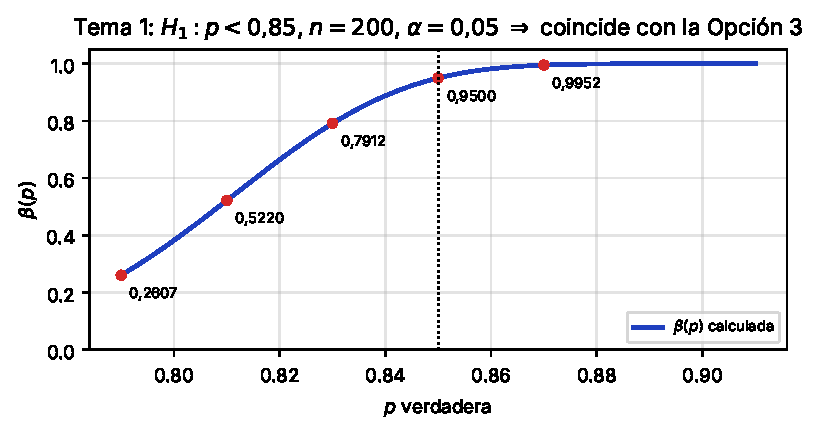
\includegraphics[width=0.78\textwidth]{fig/t1beta.pdf}
\end{figure}
\begin{resp}
\textbf{Opción 3.} La curva es \textbf{creciente} (la prueba es unilateral izquierda), vale $1-\alpha=0{,}95$ en $p_0=0{,}85$, tiende a 1 para $p>0{,}85$ y pasa por $(0{,}79;\,0{,}26)$, como la calculada.
Se descartan: 2 y 5 (forma de campana: corresponden a una prueba bilateral); 1 y 4 (decrecientes: corresponderían a $H_1:p>0{,}85$); 6 (creciente, pero en $p=0{,}79$ vale $\approx0{,}36$ y no $0{,}26$, y ya está casi en 1 en $p=0{,}85$ cuando debería valer $0{,}95$).
\end{resp}

\inciso{d) IC del 95\,\% para la proporción de pedidos a tiempo}
\paso{Planteo.} $n$ es grande, así que por el TCL se usa $\hat p\pm z_{0,025}\sqrt{\hat p(1-\hat p)/n}$. En el IC se usa $\hat p$ (no $p_0$), porque no se supone ningún valor de $p$.
\[
0{,}80\pm1{,}96\sqrt{\frac{0{,}8\cdot0{,}2}{200}}=0{,}80\pm1{,}96\,(0{,}0283)=0{,}80\pm0{,}0554\ \Rightarrow\ \res{0{,}7446\le p\le0{,}8554}
\]
\paso{Comparación con b).} El IC \emph{bilateral} contiene a 0,85, pero la prueba rechazó $H_0$. \textbf{No hay contradicción}, por dos motivos:
\begin{enumerate}
\item La prueba es \emph{unilateral} con $\alpha=0{,}05$. Lo que le corresponde es la \textbf{cota superior} del 95\,\%: $p\le0{,}80+1{,}6449\,(0{,}0283)=0{,}8465<0{,}85$, que sí excluye a 0,85, coherente con el rechazo.
\item En la prueba el error estándar se calcula con $p_0$ (0,0252) y en el IC con $\hat p$ (0,0283). Para proporciones, la dualidad IC--prueba es solo aproximada.
\end{enumerate}

\inciso{e) Tamaño de muestra para un error máximo $E=0{,}03$ con 95\,\%}
\paso{Fórmula.} De $E=z_{\alpha/2}\sqrt{p(1-p)/n}$ se despeja $n=\dfrac{z_{\alpha/2}^2\,p(1-p)}{E^2}$.

\paso{Para garantizarlo para cualquier $p$.} Como $p(1-p)\le\frac14$ (el máximo está en $p=\frac12$):
\[
n=\frac{1{,}96^2\cdot0{,}25}{0{,}03^2}=1067{,}1\ \Rightarrow\ \res{n=1068}
\]
\paso{Usando la estimación previa $\hat p=0{,}80$.} $n=\frac{1{,}96^2\cdot0{,}8\cdot0{,}2}{0{,}03^2}=682{,}95\Rightarrow683$.
\begin{resp}
Para \textbf{garantizar} el error máximo de 3 puntos sin depender del valor de $p$: $n=1068$. Si se acepta como estimación previa el $\hat p=0{,}80$ de esta muestra, alcanza con $n=683$, o sea 483 pedidos más que los 200 ya observados.
\end{resp}

% =====================================================================
\newpage
\section{Parcial 2025 --- Tema 2}

\subsection{Ejercicio 1 --- Distribución conjunta con regla de parada}
\begin{enun}
Igual que en el Tema 1, pero con 5 activos (A), 2 en reposo (R) y 3 desconectados (D). $X$ = activos observados; $Y$ = \emph{desconectados} observados.
c) Si hay al menos un activo, probabilidad de que \emph{no} se haya observado un nodo desconectado.
\end{enun}
\begin{metodo}
El mismo que en el Tema 1: secuencias posibles, regla del producto y armado de la tabla.
\end{metodo}
\inciso{a) Matriz de probabilidad conjunta}
\begin{center}
\renewcommand{\arraystretch}{1.25}
\begin{tabular}{@{}lllcc@{}}
\toprule
Secuencia & Cálculo & Probabilidad & $x$ & $y$\\\midrule
R & $\frac{2}{10}$ & $0{,}2000$ & 0 & 0\\
D & $\frac{3}{10}$ & $0{,}3000$ & 0 & 1\\
A R & $\frac{5}{10}\cdot\frac{2}{9}=\frac19$ & $0{,}1111$ & 1 & 0\\
A D & $\frac{5}{10}\cdot\frac{3}{9}=\frac16$ & $0{,}1667$ & 1 & 1\\
A A R & $\frac{5}{10}\cdot\frac{4}{9}\cdot\frac{2}{8}=\frac1{18}$ & $0{,}0556$ & 2 & 0\\
A A D & $\frac{5}{10}\cdot\frac{4}{9}\cdot\frac{3}{8}=\frac1{12}$ & $0{,}0833$ & 2 & 1\\
A A A & $\frac{5}{10}\cdot\frac{4}{9}\cdot\frac{3}{8}=\frac1{12}$ & $0{,}0833$ & 3 & 0\\\bottomrule
\end{tabular}
\qquad
\begin{tabular}{@{}c|cc|c@{}}
\toprule
$p(x,y)$ & $y=0$ & $y=1$ & $p_X$\\\midrule
$x=0$ & 0,2000 & 0,3000 & \textbf{0,5000}\\
$x=1$ & 0,1111 & 0,1667 & \textbf{0,2778}\\
$x=2$ & 0,0556 & 0,0833 & \textbf{0,1389}\\
$x=3$ & 0,0833 & 0 & \textbf{0,0833}\\\midrule
$p_Y$ & \textbf{0,4500} & \textbf{0,5500} & 1\\\bottomrule
\end{tabular}
\end{center}
(Numéricamente la tabla coincide con la del Tema 1, porque los roles de R y D se intercambian junto con la definición de $Y$.)

\inciso{b) Covarianza e independencia}
$\E(X)=\frac{29}{36}=0{,}8056$, \ $\E(Y)=0{,}55$, \ $\E(XY)=1\cdot\frac16+2\cdot\frac1{12}=\frac13$:
\[
\Cov(X,Y)=\frac13-\frac{29}{36}\cdot\frac{11}{20}=\res{-\frac{79}{720}=-0{,}1097}\neq0\ \Rightarrow\ \textbf{no son independientes}.
\]
(Además $p(3,1)=0\neq p_X(3)p_Y(1)$.) La covarianza es negativa: cuantos más activos se observan, menos probable es que aparezca un desconectado, y el desconectado corta la observación.

\inciso{c) Probabilidad condicional}
Lo pedido es $P(Y=0\,|\,X\ge1)$:
\[
P(Y=0\,|\,X\ge1)=\frac{p(1,0)+p(2,0)+p(3,0)}{1-p_X(0)}=\frac{\frac19+\frac1{18}+\frac1{12}}{\frac12}=\frac{45/180}{1/2}=\res{0{,}5000}
\]

\subsection{Ejercicio 2 --- Verdadero o falso}
\inciso{a) FALSA}
Es la misma proposición del Tema 1: $\Cov(h-X,X)=-\V(X)\le0$, y vale 0 si $X$ es degenerada. Ver la sección 1.2.

\inciso{b) FALSA: no siempre hace falta una muestra preliminar}
\paso{Planteo.} El error máximo es $E=z_{\alpha/2}\sqrt{p(1-p)/n}$. La función $g(p)=p(1-p)$ tiene $g'(p)=1-2p=0$ en $p=\frac12$ y $g''=-2<0$, así que es un máximo: $p(1-p)\le\frac14$ para todo $p$. Entonces
\[
E\le z_{\alpha/2}\sqrt{\frac{1}{4n}}\le\varepsilon\iff n\ge\frac{z_{\alpha/2}^2}{4\varepsilon^2}.
\]
\begin{resp}
\textbf{Falsa.} Con el criterio conservador ($p=0{,}5$) se garantiza el error $\le\varepsilon$ para \emph{cualquier} $p$, sin muestra preliminar. Por ejemplo, $\varepsilon=0{,}03$ y 95\,\% dan $n=1{,}96^2/(4\cdot0{,}03^2)=1067{,}1\to1068$.
La muestra preliminar (o un dato histórico) solo sirve para obtener un $n$ menor; no es obligatoria.
\end{resp}

\subsection{Ejercicio 3 --- Prueba para la media con $\sigma$ conocido}
\begin{enun}
Tornillos con diámetro nominal 20,00 mm. Se quiere saber si hay que ajustar la maquinaria: $n=36$, $\xb=20{,}15$ mm, $\sigma=0{,}40$ mm.
a) Planteo con $\alpha=0{,}05$. \ b) Conclusión, error posible y valor $P$. \ c) Curva de $\beta$. \ d) IC 95\,\% para $\mu$. \ e) $n$ para detectar $\mu=20{,}1$ con probabilidad 0,80.
\end{enun}
\begin{metodo}
Prueba $Z$ para la media con $\sigma$ conocido. Con $n=36\ge30$, el \textbf{TCL} garantiza que $\Xb\approx\Nor(\mu;\sigma^2/n)$ aunque el diámetro no sea normal. Error estándar: $\sigma/\sqrt n=0{,}40/6=0{,}0667$.
\end{metodo}
\inciso{a) Planteo}
``Verificar si es necesario ajustar'' significa detectar un desvío \textbf{para cualquier lado}, así que la prueba es \textbf{bilateral}:
\[
H_0:\mu=20\qquad\text{vs.}\qquad H_1:\mu\neq20;\qquad Z=\frac{\Xb-20}{0{,}40/\sqrt{36}}\ \overset{H_0}{\approx}\ \Nor(0;1).
\]
Región de rechazo: $|Z|>z_{0,025}=1{,}96$. En unidades de $\xb$: $\xb<19{,}8693$ o $\xb>20{,}1307$.

\inciso{b) Conclusión, error y valor $P$}
\[
z_0=\frac{20{,}15-20}{0{,}0667}=\res{2{,}25}>1{,}96\ \Rightarrow\ \textbf{se rechaza }H_0.
\]
\begin{resp}
Con $\alpha=0{,}05$ hay evidencia de que el diámetro medio difiere de 20 mm: hay que ajustar la máquina.
\textbf{Error posible:} tipo I, es decir, ajustar la máquina cuando en realidad está bien calibrada ($\mu=20$). Su probabilidad es como máximo 0,05.
\textbf{Valor $P$} $=2[1-\Phi(2{,}25)]=2(0{,}0122)=\res{0{,}0244}<0{,}05$, así que se rechaza: coincide con la decisión.
\end{resp}

\inciso{c) Curva de probabilidad de error tipo II}
Con $d=(\mu-20)/0{,}0667$: \ $\beta(\mu)=\Phi(1{,}96-d)-\Phi(-1{,}96-d)$.
\begin{center}
\begin{tabular}{@{}lccccc@{}}
\toprule
$\mu$ & 19,8 & 19,9 & 20,0 & 20,1 & 20,2\\\midrule
$\beta(\mu)$ & 0,1492 & 0,6770 & 0,9500 & 0,6770 & 0,1492\\\bottomrule
\end{tabular}
\end{center}
\begin{figure}[h]
\centering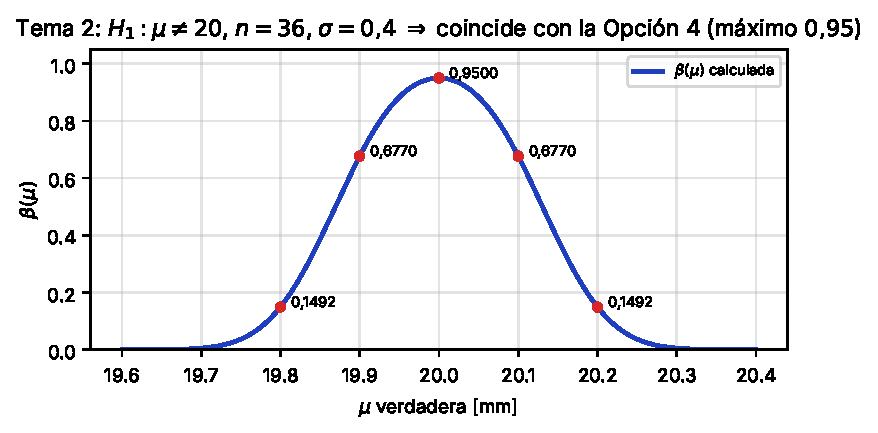
\includegraphics[width=0.78\textwidth]{fig/t2beta.pdf}
\end{figure}
\begin{resp}
\textbf{Opción 4.} Es una campana \textbf{simétrica} alrededor de $\mu_0=20$ (prueba bilateral), con máximo $1-\alpha=0{,}95$ en $\mu=20$, y vale $\approx0{,}15$ en 19,8 y en 20,2.
Se descartan: 2 (campana con máximo 0,90, que correspondería a $\alpha=0{,}10$); 1, 3, 5 y 6 (monótonas: corresponden a pruebas unilaterales).
\end{resp}

\inciso{d) IC del 95\,\% para $\mu$}
Con $\sigma$ conocido y $n=36$:
\[
20{,}15\pm1{,}96\,(0{,}0667)=20{,}15\pm0{,}1307\ \Rightarrow\ \res{20{,}0193\le\mu\le20{,}2807\ \text{mm}}
\]
El valor 20 \textbf{no} está en el intervalo, lo que coincide con el rechazo de b). Por la dualidad, una prueba bilateral con nivel $\alpha$ rechaza $H_0$ exactamente cuando $\mu_0$ queda fuera del IC del $(1-\alpha)$.

\inciso{e) Tamaño de muestra}
Se pide potencia 0,80 (o sea $\beta=0{,}20$) cuando $\mu=20{,}1$ ($\delta=0{,}1$), con la misma prueba bilateral y $\alpha=0{,}05$. Los valores críticos son $z_{0,025}=1{,}96$ y $z_{0,20}=0{,}8416$:
\[
n\approx\frac{(z_{\alpha/2}+z_\beta)^2\sigma^2}{\delta^2}=\frac{(1{,}96+0{,}8416)^2\,(0{,}40)^2}{0{,}1^2}=125{,}59\ \Rightarrow\ \res{n=126}
\]
Comprobación: con $n=126$ la potencia es 0,8013 \checkmark; con $n=125$ sería 0,7982, que no alcanza.

% =====================================================================
\newpage
\part{Modelos de Segundo Parcial}
% =====================================================================
\section{Modelo A}

\subsection{Ejercicio 1 --- Cajas registradoras}
\begin{enun}
Hay 3 cajas. Dos clientes eligen cada uno una caja al azar, en forma independiente. $X$ = número de clientes que eligen la caja 1; $Y$ = número que eligen la caja 2.
a) Tabla conjunta. \ b) ¿Independientes? \ c) ¿Misma distribución? \ d) $\Cov(X,Y)$.
\end{enun}
\begin{metodo}
Cada cliente elige caja 1, 2 o 3 con probabilidad $\frac13$ cada una, de forma independiente. Hay $3^2=9$ resultados equiprobables, cada uno con probabilidad $\frac19$, y se cuenta cuántos dan cada par $(x,y)$. Es una distribución trinomial (multinomial) con $n=2$.
\end{metodo}
\inciso{a) Tabla conjunta}
Resultados (caja del cliente 1, caja del cliente 2):
(1,1): $x=2,y=0$; \ (2,2): $x=0,y=2$; \ (3,3): $x=0,y=0$; \ (1,2),(2,1): $x=1,y=1$; \ (1,3),(3,1): $x=1,y=0$; \ (2,3),(3,2): $x=0,y=1$.
\begin{center}
\renewcommand{\arraystretch}{1.3}
\begin{tabular}{@{}c|ccc|c@{}}
\toprule
$p(x,y)$ & $y=0$ & $y=1$ & $y=2$ & $p_X(x)$\\\midrule
$x=0$ & $1/9$ & $2/9$ & $1/9$ & $\mathbf{4/9}$\\
$x=1$ & $2/9$ & $2/9$ & $0$ & $\mathbf{4/9}$\\
$x=2$ & $1/9$ & $0$ & $0$ & $\mathbf{1/9}$\\\midrule
$p_Y(y)$ & $\mathbf{4/9}$ & $\mathbf{4/9}$ & $\mathbf{1/9}$ & 1\\\bottomrule
\end{tabular}
\end{center}
\inciso{b) Independencia}
$p(2,2)=0$, pero $p_X(2)\,p_Y(2)=\frac19\cdot\frac19=\frac1{81}\neq0$. \textbf{No son independientes}: hay solo dos clientes, así que si los dos van a la caja 1, ninguno va a la caja 2.

\inciso{c) ¿Misma distribución?}
\textbf{Sí}: las dos marginales son $(4/9;\,4/9;\,1/9)$, es decir, $X\sim Y\sim\mathrm{Bin}(2;\,1/3)$. Tienen la misma distribución, pero no son la misma variable ni son independientes.

\inciso{d) Covarianza}
$\E(X)=\E(Y)=2\cdot\frac13=\frac23$. \quad $\E(XY)$: solo aporta la celda $(1,1)$: $\E(XY)=1\cdot1\cdot\frac29=\frac29$.
\[
\Cov(X,Y)=\frac29-\frac23\cdot\frac23=\frac29-\frac49=\res{-\frac29=-0{,}2222}
\]
(Coincide con la fórmula de la multinomial, $\Cov=-n\,p_1p_2=-2\cdot\frac13\cdot\frac13$.)

\subsection{Ejercicio 2 --- Tamaño de muestra para una proporción}
\begin{enun}
¿Cuántos clientes hay que encuestar para que la fracción muestral de insatisfechos se desvíe a lo sumo 0,15 de la poblacional, con probabilidad no menor a 0,98? Definir variables, distribución y parámetros; justificar con propiedades y teoremas.
\end{enun}
\begin{metodo}
$X_i=1$ si el cliente $i$ está insatisfecho y 0 si no: $X_i\sim$ Bernoulli$(p)$, independientes.
$T=\sum X_i\sim\mathrm{Bin}(n;p)$ y $\hat P=T/n$, con $\E(\hat P)=p$ y $\V(\hat P)=p(1-p)/n$ (propiedades de la esperanza y la varianza).
Por el \textbf{TCL}, para $n$ grande, $\hat P\approx\Nor\big(p;\,p(1-p)/n\big)$. Como $p$ es desconocido, se usa el peor caso $p(1-p)\le\frac14$.
\end{metodo}
\paso{Planteo.}
\[
P\big(|\hat P-p|\le0{,}15\big)\ge0{,}98\iff P\Big(|Z|\le\frac{0{,}15}{\sqrt{p(1-p)/n}}\Big)\ge0{,}98\iff\frac{0{,}15\sqrt n}{\sqrt{p(1-p)}}\ge z_{0,01}=2{,}3263.
\]
\paso{Despeje.} $n\ge\dfrac{z_{0,01}^2\,p(1-p)}{0{,}15^2}$. Como $p$ es desconocido, se toma el peor caso $p(1-p)=\frac14$, que vale para cualquier $p$:
\[
n\ge\frac{2{,}3263^2\cdot0{,}25}{0{,}0225}=60{,}13\ \Rightarrow\ \res{n=61}
\]
\begin{resp}
Hay que encuestar \textbf{61 clientes}. Con ese $n$ se cumple para cualquier valor de $p$.
Si se usara la desigualdad de Chebyshev, que no requiere aproximación normal, se obtendría $P(|\hat P-p|>0{,}15)\le\frac{1}{4n(0{,}15)^2}\le0{,}02$, de donde $n\ge556$: más conservador.
\end{resp}

\subsection{Ejercicio 3 --- Redacción de la conclusión}
\begin{enun}
$H_0$: el método no es efectivo. $H_1$: el método es efectivo. Si se \emph{rechaza} $H_0$, ¿está bien la conclusión ``No hay evidencia significativa para concluir que el método no es efectivo''?
\end{enun}
\begin{resp}
\textbf{No está bien expresada.} Rechazar $H_0$ significa que los datos aportan evidencia significativa \emph{a favor de $H_1$}. La frase dada habla de ``falta de evidencia'', que es el lenguaje de \emph{no rechazar}, y además se refiere a la afirmación de $H_0$ en vez de a la de $H_1$.
\textbf{Corrección:} ``Hay evidencia significativa (al nivel $\alpha$) para concluir que el método \emph{es} efectivo.''
\end{resp}

\subsection{Ejercicio 4 --- Nivel de significación y error tipo II}
\begin{enun}
$\sigma=8{,}4$; $H_0:\mu=80$ vs.\ $H_1:\mu<80$; $n=100$. Se rechaza $H_0$ si $\xb\le78{,}2$.
a) Nivel de significación. \ b) Error tipo II en contexto y su probabilidad si $\mu$ difiere de 80 en 1,3. \ c) Conclusión si el valor $P$ es 0,011.
\end{enun}
\begin{metodo}
Con $n=100$, por el TCL $\Xb\approx\Nor(\mu;\,\sigma^2/n)$, con $\sigma/\sqrt n=8{,}4/10=0{,}84$. $\alpha$ y $\beta$ se calculan como áreas bajo esa normal, usando la región de rechazo dada.
\end{metodo}
\inciso{a) Nivel de significación}
\[
\alpha=P(\Xb\le78{,}2\,|\,\mu=80)=\Phi\Big(\frac{78{,}2-80}{0{,}84}\Big)=\Phi(-2{,}1429)=\res{0{,}0161}
\]
\inciso{b) Error tipo II}
\textbf{Significado:} no rechazar $H_0$ (concluir que la media es 80) cuando en realidad es menor.
Como $H_1$ es $\mu<80$, ``difiere en 1,3'' significa $\mu=80-1{,}3=78{,}7$:
\[
\beta=P(\Xb>78{,}2\,|\,\mu=78{,}7)=1-\Phi\Big(\frac{78{,}2-78{,}7}{0{,}84}\Big)=1-\Phi(-0{,}5952)=\res{0{,}7242}
\]
Esta prueba tiene poca potencia (0,2758) para detectar una diferencia de 1,3.

\inciso{c) Valor $P=0{,}011$}
Se rechaza $H_0$ si $P\le\alpha$. Con el nivel de esta prueba, $\alpha=0{,}0161$, se tiene $0{,}011<0{,}0161$: \textbf{se rechaza $H_0$}. Hay evidencia de que $\mu<80$. (Con $\alpha=0{,}05$ también se rechazaría; con $\alpha=0{,}01$, no.)

\subsection{Ejercicio 5 --- Verdadero o falso}
\inciso{a) VERDADERA}
$Y=a\Xb_1+(1-a)\Xb_2$ con $n_2=4n_1$. Por linealidad, y porque $\E(\Xb_i)=\mu$:
\[
\E(Y)=a\mu+(1-a)\mu=\mu\quad\Rightarrow\ \text{insesgado para todo }a.
\]
Las muestras son independientes, así que
\[
\V(Y)=a^2\frac{\sigma^2}{n_1}+(1-a)^2\frac{\sigma^2}{4n_1}=\frac{\sigma^2}{n_1}\Big[a^2+\frac{(1-a)^2}{4}\Big].
\]
Se minimiza derivando: $\frac{d}{da}\big[a^2+\frac{(1-a)^2}4\big]=2a-\frac{(1-a)}{2}=0\Rightarrow4a=1-a\Rightarrow\res{a=\frac15}$. La derivada segunda es $2+\frac12>0$, así que es un mínimo.
(Es el promedio ponderado por los tamaños: $a=\frac{n_1}{n_1+n_2}=\frac15$.)

\inciso{b) VERDADERA}
La longitud del IC con $\sigma$ conocido es $L=2z_{\alpha/2}\sigma/\sqrt n$. Para tener $L'=L/2$ con la misma confianza: $\frac{1}{\sqrt{n'}}=\frac{1}{2\sqrt n}\Rightarrow\sqrt{n'}=2\sqrt n\Rightarrow n'=4n$. Hay que \textbf{cuadruplicar} $n$.

\inciso{c) FALSA}
La población es normal, $\sigma$ es desconocido y $n=9$ es chico, así que corresponde $t$ con 8 g.l.: $t_{0,015;\,8}=2{,}6338$.
\[
6\pm2{,}6338\cdot\frac{0{,}12}{\sqrt9}=6\pm0{,}1054\ \Rightarrow\ \res{(5{,}8946;\ 6{,}1054)}
\]
El intervalo del enunciado, $(5{,}9132;\,6{,}0868)$, tiene semiamplitud $0{,}0868=2{,}1701\cdot0{,}04$: se calculó con $z_{0,015}=2{,}1701$, que no corresponde porque $\sigma$ es desconocido. Por eso la afirmación es \textbf{falsa}.

% =====================================================================
\newpage
\section{Modelo B}

\subsection{Problema 1 --- Circuito de tres componentes}
\begin{enun}
A y B en serie, y esa rama en paralelo con C. Los componentes son independientes y cada uno funciona con probabilidad 0,92. $X$ = cantidad de componentes que funcionan; $Y=1$ si el circuito funciona y $0$ si no.
a) $p_{XY}(x,y)$. \ b) Si funciona a lo sumo un componente, probabilidad de que el circuito no funcione. \ c) Coeficiente de correlación. \ d) De 100 circuitos, probabilidad de que funcionen al menos 96.
\end{enun}
\begin{metodo}
El circuito funciona si y solo si $(A\cap B)\cup C$. Se recorren los $2^3=8$ estados (independencia: producto de probabilidades, con $q=0{,}92$ y $1-q=0{,}08$) y se anota $(x,y)$. Además, $X\sim\mathrm{Bin}(3;\,0{,}92)$.
\end{metodo}
\inciso{a) Función de probabilidad conjunta}
\begin{center}
\renewcommand{\arraystretch}{1.25}
\begin{tabular}{@{}lccc@{}}
\toprule
Estado (funcionan) & Probabilidad & $x$ & $y$\\\midrule
ninguno & $0{,}08^3=0{,}000512$ & 0 & 0\\
solo A, o solo B & $2\cdot0{,}92\cdot0{,}08^2=0{,}011776$ & 1 & 0\\
solo C & $0{,}92\cdot0{,}08^2=0{,}005888$ & 1 & 1\\
AB, AC o BC & $3\cdot0{,}92^2\cdot0{,}08=0{,}203136$ & 2 & 1\\
ABC & $0{,}92^3=0{,}778688$ & 3 & 1\\\bottomrule
\end{tabular}
\qquad
\begin{tabular}{@{}c|cc|c@{}}
\toprule
$p$ & $y=0$ & $y=1$ & $p_X$\\\midrule
$x=0$ & 0,000512 & 0 & 0,000512\\
$x=1$ & 0,011776 & 0,005888 & 0,017664\\
$x=2$ & 0 & 0,203136 & 0,203136\\
$x=3$ & 0 & 0,778688 & 0,778688\\\midrule
$p_Y$ & 0,012288 & 0,987712 & 1\\\bottomrule
\end{tabular}
\end{center}
Con dos componentes funcionando, el circuito siempre funciona: si son A y B, por la rama en serie; si uno de los dos es C, por C.

\inciso{b) $P(Y=0\,|\,X\le1)$}
\[
P(Y=0\,|\,X\le1)=\frac{p(0,0)+p(1,0)}{p_X(0)+p_X(1)}=\frac{0{,}000512+0{,}011776}{0{,}000512+0{,}017664}=\frac{0{,}012288}{0{,}018176}=\res{0{,}6761}
\]
\inciso{c) Coeficiente de correlación}
$\E(X)=3(0{,}92)=2{,}76$; $\V(X)=3(0{,}92)(0{,}08)=0{,}2208$.
$\E(Y)=0{,}987712$; $\V(Y)=0{,}987712\cdot0{,}012288=0{,}012137$.
$\E(XY)=1(0{,}005888)+2(0{,}203136)+3(0{,}778688)=2{,}748224$.
\[
\Cov=2{,}748224-2{,}76\cdot0{,}987712=0{,}022139;\qquad
\rho=\frac{0{,}022139}{\sqrt{0{,}2208\cdot0{,}012137}}=\res{0{,}4277}
\]
\textbf{Interpretación:} hay una asociación lineal positiva y moderada. Cuantos más componentes funcionan, más probable es que funcione el circuito. No es una relación lineal fuerte porque $Y$ solo toma 0 o 1, y vale 1 casi siempre.

\inciso{d) Al menos 96 de 100 circuitos funcionan}
Sea $W$ = número de circuitos que funcionan, $W\sim\mathrm{Bin}(100;\,0{,}987712)$. Hay pocos fallos esperados: $n(1-p)=1{,}2288<5$, así que la aproximación normal \textbf{no} es adecuada. Se usa la de \textbf{Poisson} para la cantidad de fallas $F=100-W\approx\mathrm{Poisson}(\lambda=1{,}2288)$:
\[
P(W\ge96)=P(F\le4)=\sum_{k=0}^{4}e^{-1{,}2288}\frac{1{,}2288^k}{k!}=\res{0{,}9915}
\]
(El valor binomial exacto es 0,9920. La normal con corrección por continuidad daría 0,9985, que es peor.)

\subsection{Problema 2 --- Estimador insesgado de $a^2$}
\begin{enun}
$X_1,\dots,X_n$ m.a.\ de $X\sim U(-a;\,a)$. Demostrar que $T=\frac3n\sum X_i^2$ es un estimador insesgado de $a^2$.
\end{enun}
\begin{metodo}
Se usan la linealidad de la esperanza y que $\E(X^2)=\V(X)+\E(X)^2$, con $\V=\frac{(b-a)^2}{12}$ para la uniforme.
\end{metodo}
\paso{Paso 1.} Para $X\sim U(-a;a)$: $\E(X)=0$ y $\V(X)=\frac{(2a)^2}{12}=\frac{a^2}{3}$, así que $\E(X_i^2)=\frac{a^2}{3}$.

\paso{Paso 2.}
\[
\E(T)=\frac3n\sum_{i=1}^n\E(X_i^2)=\frac3n\cdot n\cdot\frac{a^2}{3}=a^2.\qquad\blacksquare
\]
Como $\E(T)=a^2$ para todo $a$, $T$ es \textbf{insesgado} para $a^2$.

\subsection{Problema 3 --- Distancia de frenado}
\begin{enun}
$n=20$ pruebas, $\xb=109{,}8$ m, $s=20$ m. a) IC de nivel 0,90 para $\mu$; ¿qué información falta? b) Si $\mu=110$, ¿el gráfico de 100 intervalos corresponde a un nivel de 0,95?
\end{enun}
\inciso{a) IC 90\,\%}
\textbf{Información omitida:} que la distancia de frenado tiene distribución \textbf{normal}. Con $\sigma$ desconocido y $n=20<30$, esa suposición es la que permite usar $T=\frac{\Xb-\mu}{S/\sqrt n}\sim t_{19}$.
\[
t_{0,05;19}=1{,}7291;\qquad109{,}8\pm1{,}7291\cdot\frac{20}{\sqrt{20}}=109{,}8\pm7{,}7329\ \Rightarrow\ \res{102{,}07\le\mu\le117{,}53\ \text{m}}
\]
\inciso{b) ¿El gráfico corresponde a 95\,\%?}
\paso{Conteo.} En el gráfico hay \textbf{14 intervalos en rojo} (no contienen a la media) de 100: una cobertura del 86\,\%.

\paso{Comparación.} Con 95\,\% de confianza, la cantidad de intervalos que fallan es $F\sim\mathrm{Bin}(100;\,0{,}05)$, con media 5 y desvío 2,18. Ver 14 o más fallos tiene probabilidad $P(F\ge14)=0{,}0005$: es muy improbable.
\begin{resp}
\textbf{No corresponde} a un nivel de 0,95: con 95\,\% se esperan unos 5 intervalos fallidos, y hay 14 (86\,\% de cobertura). Además, la línea de referencia está en 109,39 y no en $\mu=110$: si el valor verdadero fuera 110, habría que contar los intervalos que no contienen a 110.
\end{resp}

\subsection{Problema 4 --- Vigas de magnesio}
\begin{enun}
La media del porcentaje de defectos no puede superar el 5\,\%. Si $\xb>5{,}5$ se detiene la producción, con probabilidad de equivocarse de 0,01. El porcentaje de defectos es normal con $\sigma^2=1$.
a) Hipótesis, estadístico, región y $n$. \ b) ¿El gráfico es una curva de potencia? \ c) Valor $P$ límite para no certificar.
\end{enun}
\inciso{a) Planteo y tamaño de muestra}
\[
H_0:\mu=5\ (\mu\le5)\qquad\text{vs.}\qquad H_1:\mu>5;\qquad Z=\frac{\Xb-5}{1/\sqrt n}\ \overset{H_0}{\sim}\ \Nor(0;1)
\]
(exacto, porque la población es normal y $\sigma$ es conocido). Región de rechazo: $\xb>5{,}5$, con $\alpha=P(\Xb>5{,}5\,|\,\mu=5)=0{,}01$.
\[
\frac{5{,}5-5}{1/\sqrt n}=z_{0,01}=2{,}3263\ \Rightarrow\ \sqrt n=4{,}6527\ \Rightarrow\ n=21{,}65\ \Rightarrow\ \res{n=22}
\]
Con $n=22$, la regla $\xb>5{,}5$ da $\alpha=0{,}0095\le0{,}01$ \checkmark. Dicho con el estadístico: se rechaza si $z_0>2{,}3263$.

\inciso{b) ¿Es una curva de potencia?}
La potencia es $\pi(\mu)=P(\Xb>5{,}5\,|\,\mu)$, que es \textbf{creciente} en $\mu$: $\pi(5)=0{,}0095$, $\pi(5{,}5)=0{,}5$, $\pi(6)=0{,}9905$.
El gráfico dado es \textbf{decreciente}: vale $\approx1$ en $\mu=5$ y $\approx0$ en $\mu=6$.
\begin{figure}[h]
\centering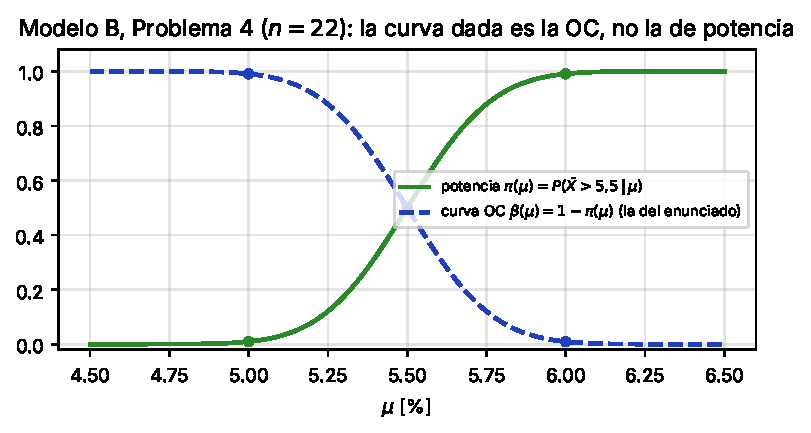
\includegraphics[width=0.78\textwidth]{fig/mbpot.pdf}
\end{figure}
\begin{resp}
\textbf{No}, es la curva \textbf{OC} $\beta(\mu)=1-\pi(\mu)$. Dos puntos lo muestran:
\begin{itemize}
\item En $\mu=5$ ($H_0$ cierta) el gráfico marca $\approx0{,}99=1-\alpha$, la probabilidad de \emph{no} rechazar. La potencia valdría $\alpha\approx0{,}01$.
\item En $\mu=6$ el gráfico marca $\approx0{,}01$, que es $\beta(6)$: la probabilidad de no detener la producción cuando la media es 6. La potencia valdría 0,99.
\end{itemize}
En $\mu=5{,}5$ las dos curvas valen 0,5.
\end{resp}

\inciso{c) Valor $P$ para no certificar}
No certificar equivale a rechazar $H_0$ (concluir que $\mu>5$), y eso ocurre si $P\le\alpha$. El valor $P$ debe ser como \textbf{máximo 0,01}: no se certifica si $P\le0{,}01$; con la regla exacta para $n=22$, $P\le0{,}0095$.

% =====================================================================
\newpage
\part{Temarios de años anteriores}
% =====================================================================
\section{Temario 1}

\subsection{Ejercicio 1 --- Cartuchos sin reposición}
\begin{enun}
Una caja tiene 3 repuestos azules, 2 rojos y 1 verde. Se extraen 2 sin reposición. $X$ = número de azules; $Y$ = número de rojos.
a) $p(x,y)$. \ b) ¿Independientes? \ c) $P(X=Y\,|\,Y\ge1)$.
\end{enun}
\begin{metodo}
Como el orden no importa para contar colores, se usa el conteo combinatorio (hipergeométrica multivariada):
$p(x,y)=\dfrac{\binom3x\binom2y\binom1{2-x-y}}{\binom62}$, con $\binom62=15$.
\end{metodo}
\inciso{a) Matriz conjunta}
$(0,0)$: harían falta 2 verdes y hay solo 1, así que vale 0. \ $(0,1)$: $\binom21\binom11=2$. \ $(0,2)$: $\binom22=1$. \ $(1,0)$: $\binom31\binom11=3$. \ $(1,1)$: $\binom31\binom21=6$. \ $(2,0)$: $\binom32=3$.
\begin{center}
\renewcommand{\arraystretch}{1.3}
\begin{tabular}{@{}c|ccc|c@{}}
\toprule
$p(x,y)$ & $y=0$ & $y=1$ & $y=2$ & $p_X(x)$\\\midrule
$x=0$ & 0 & $2/15$ & $1/15$ & $\mathbf{3/15}$\\
$x=1$ & $3/15$ & $6/15$ & 0 & $\mathbf{9/15}$\\
$x=2$ & $3/15$ & 0 & 0 & $\mathbf{3/15}$\\\midrule
$p_Y(y)$ & $\mathbf{6/15}$ & $\mathbf{8/15}$ & $\mathbf{1/15}$ & 1\\\bottomrule
\end{tabular}
\end{center}
\inciso{b) Independencia}
$p(0,0)=0$, pero $p_X(0)\,p_Y(0)=\frac3{15}\cdot\frac6{15}=0{,}08\neq0$. \textbf{No son independientes}.

\inciso{c) $P(X=Y\,|\,Y\ge1)$}
Con $Y\ge1$, el único par con $X=Y$ posible es $(1,1)$ ($(2,2)$ es imposible):
\[
P(X=Y\,|\,Y\ge1)=\frac{p(1,1)}{p_Y(1)+p_Y(2)}=\frac{6/15}{9/15}=\res{\frac23=0{,}6667}
\]

\subsection{Ejercicio 2 --- Combinación lineal y suma de variables}
\begin{enun}
$\E(X)=\E(Y)=0$, $\V(X)=2$, $\V(Y)=4$, $\Cov(X,Y)=-2$.
a) $\V(W)$ con $W=5X-3Y+8$. \ b) $T=Y_1+\dots+Y_n$ (m.a.\ de $Y$): ¿se puede hallar $n$ para que $P(|T-\E(T)|>35)\ge0{,}12$?
\end{enun}
\inciso{a) Varianza de una combinación lineal}
\[
\V(5X-3Y+8)=5^2\V(X)+(-3)^2\V(Y)+2(5)(-3)\Cov(X,Y)
\]
\[
=25(2)+9(4)-30(-2)=50+36+60=\res{146}
\]
(La constante 8 no cambia la varianza.)

\inciso{b) Tamaño $n$}
\paso{Paso 1 --- Momentos de $T$.} Las $Y_i$ son iid, así que $\E(T)=n\cdot0=0$ y $\V(T)=n\cdot4=4n$.

\paso{Paso 2 --- Qué herramienta sirve.} No se conoce la distribución de $Y$. Chebyshev da solo una \emph{cota superior}, $P(|T|>35)\le\frac{4n}{35^2}$, y no sirve para asegurar ``al menos 0,12''. Lo que permite calcularlo es el \textbf{TCL}: para $n$ grande, $T\approx\Nor(0;\,4n)$.

\paso{Paso 3 --- Despeje.}
\[
P(|T|>35)\approx2\Big[1-\Phi\Big(\frac{35}{2\sqrt n}\Big)\Big]\ge0{,}12\iff\Phi\Big(\frac{35}{2\sqrt n}\Big)\le0{,}94
\]
\[
\iff\frac{35}{2\sqrt n}\le z_{0,06}=1{,}5548
\]
\[
\sqrt n\ge\frac{35}{2(1{,}5548)}=11{,}2557\ \Rightarrow\ n\ge126{,}69\ \Rightarrow\ \res{n\ge127}
\]
Comprobación: con $n=127$ la probabilidad es 0,1205 \checkmark; con $n=126$ es 0,1190, que no alcanza.
\begin{resp}
Sí es posible, \textbf{en forma aproximada, con el TCL}: hace falta $n\ge127$. Como $n$ resulta grande, el uso del TCL es razonable. (La probabilidad crece con $n$, porque el desvío de $T$ crece como $2\sqrt n$.)
\end{resp}

\subsection{Ejercicio 3 --- Cuántos registros más para el IC}
\begin{enun}
D.D.B.O.\ normal con $\sigma$ conocido. Con $n=25$ días, el IC del 90\,\% tuvo amplitud $\varepsilon$. Se quiere un IC de al menos 98\,\% con amplitud $\varepsilon/2$. ¿Cuántos registros más hacen falta como mínimo?
\end{enun}
\begin{metodo}
Con $\sigma$ conocido y población normal, la amplitud del IC es $A=2z_{\alpha/2}\,\sigma/\sqrt n$. Se plantea la condición nueva en función de la amplitud anterior y $\sigma$ se cancela.
\end{metodo}
\paso{Paso 1.} Amplitud anterior: $\varepsilon=2\,z_{0,05}\,\frac{\sigma}{\sqrt{25}}=2(1{,}6449)\frac{\sigma}{5}$.

\paso{Paso 2.} Condición nueva: $2\,z_{0,01}\frac{\sigma}{\sqrt n}\le\frac{\varepsilon}{2}=\frac{1{,}6449\,\sigma}{5}$, con $z_{0,01}=2{,}3263$:
\[
\frac{2(2{,}3263)}{\sqrt n}\le\frac{1{,}6449}{5}\ \Rightarrow\ \sqrt n\ge\frac{10\,(2{,}3263)}{1{,}6449}=14{,}1425\ \Rightarrow\ n\ge200{,}01\ \Rightarrow\ n=201.
\]
\begin{resp}
Hacen falta $n=201$ registros en total, es decir, \textbf{$201-25=176$ registros más}.
(El resultado queda justo en el límite de 200. Con los valores redondeados de tabla, 2,326 y 1,645, daría 199,93, o sea 200 registros y 175 más. Por eso conviene usar 4 decimales, como pide el parcial.)
\end{resp}

\subsection{Ejercicio 4 --- Prueba para la varianza (arenas)}
\begin{enun}
Las arenas de buena calidad tienen varianza de material perdido menor que 2. Con 10 muestras se obtuvo $s^2=1{,}6$. ¿Hay evidencia significativa para afirmar que la arena puede usarse? Parámetro, hipótesis, errores en contexto, estadístico, suposiciones y conclusión.
\end{enun}
\begin{metodo}
Prueba para una varianza. Se supone que el material perdido tiene distribución \textbf{normal} y que las muestras son independientes. Así, $\frac{(n-1)S^2}{\sigma^2}\sim\chis_{n-1}$.
Como no se da $\alpha$, se usa $\alpha=0{,}05$ y se informa también el valor $P$.
\end{metodo}
\paso{Parámetro:} $\sigma^2$, la varianza del material perdido (g/muestra) en el ensayo a 10\,000 psi.

\paso{Hipótesis.} Lo que se quiere demostrar es que la arena es apta, o sea $\sigma^2<2$, y eso va en $H_1$:
\[
H_0:\sigma^2=2\ (\sigma^2\ge2)\qquad\text{vs.}\qquad H_1:\sigma^2<2.
\]
\paso{Errores en contexto.}
\begin{itemize}
\item \textbf{Tipo I:} concluir que la arena es apta ($\sigma^2<2$) cuando no lo es. Se usaría una arena inadecuada en los pozos: es el error grave, y por eso es el que se controla con $\alpha$.
\item \textbf{Tipo II:} no encontrar evidencia de aptitud cuando la arena sí es apta. Se descartaría una arena buena.
\end{itemize}
\paso{Estadístico:} $\chis=\frac{(n-1)S^2}{\sigma_0^2}\ \overset{H_0}{\sim}\ \chis_{9}$. Región de rechazo: $\chis_0<\chis_{0,95;\,9}=3{,}3251$.

\paso{Cálculo:} $\chis_0=\frac{9\cdot1{,}6}{2}=7{,}2>3{,}3251$, así que \textbf{no se rechaza $H_0$}. Valor $P=P(\chis_9\le7{,}2)=0{,}3837$.
\begin{resp}
No hay evidencia significativa para afirmar que $\sigma^2<2$. Aunque $s^2=1{,}6<2$, con solo 10 muestras esa diferencia puede deberse al azar ($P=0{,}38$). \textbf{No se puede asegurar que la arena sea apta.}
\end{resp}

\subsection{Ejercicio 5 --- Lectura de una curva de potencia}
\begin{enun}
El gráfico anexo es la potencia de una prueba para la proporción $p$ (muestra grande). Deducir: i) $H_0$ y $H_1$; ii) el nivel de significación; iii) la probabilidad de no rechazar $H_0$ si $p=0{,}7$. ¿Es una probabilidad de error?
\end{enun}
\begin{metodo}
La potencia $\pi(p)=P(\text{rechazar }H_0\,|\,p)$ vale $\alpha$ en el valor de $H_0$ (es su mínimo) y crece hacia 1 a medida que $p$ se aleja de $p_0$. La forma (simétrica o monótona) indica si la prueba es bilateral o unilateral.
\end{metodo}
En la hoja de gráficos hay tres curvas distintas, cada una repetida dos veces. Todas son simétricas, con mínimo en $p=0{,}5$ y potencia 1 en los extremos. Se resuelven las tres:
\begin{center}
\small\renewcommand{\arraystretch}{1.3}
\begin{tabular}{@{}lccc@{}}
\toprule
& Gráficos 1 y 2 (fila 1) & Gráficos 3 y 4 (fila 2) & Gráficos 5 y 6 (fila 3)\\\midrule
i) Hipótesis & \multicolumn{3}{c}{$H_0:p=0{,}5$ \ vs.\ $H_1:p\neq0{,}5$ (bilateral, por la simetría)}\\
ii) $\alpha=\pi(0{,}5)$ & $0{,}10$ & $0{,}05$ & $0{,}05$\\
Potencia en $p=0{,}7$ & $\approx0{,}90$ & $\approx0{,}83$ & $\approx0{,}89$\\
iii) $P(\text{no rechazar}\,|\,p=0{,}7)$ & $\approx0{,}10$ & $\approx0{,}17$ & $\approx0{,}11$\\\bottomrule
\end{tabular}
\end{center}
\begin{resp}
i) $H_0:p=0{,}5$ vs.\ $H_1:p\neq0{,}5$: la curva es simétrica con mínimo en 0,5. \quad
ii) $\alpha$ es la potencia en $p_0=0{,}5$, el mínimo de la curva. \quad
iii) $P(\text{no rechazar}\,|\,p=0{,}7)=1-\pi(0{,}7)=\beta(0{,}7)$. \textbf{Sí es una probabilidad de error}: con $p=0{,}7$, $H_0$ es falsa, y no rechazarla es un \textbf{error de tipo II}.
(Consistencia: las tres curvas corresponden aproximadamente a $n\approx50$ con $\alpha=0{,}10$, $n\approx50$ con $\alpha=0{,}05$ y $n\approx60$ con $\alpha=0{,}05$. Por eso la fila 1 tiene más potencia que la 2 con el mismo $n$: tiene un $\alpha$ mayor.)
\end{resp}

% =====================================================================
\newpage
\section{Temario 2}

\subsection{Problema 1 --- Bolillas: conjunta, correlación y TCL}
\begin{enun}
Una caja tiene 3 bolillas rojas, 3 blancas y 4 negras. Se extraen 2 sin reemplazo y después se devuelven. $X=1$ si la primera es roja (0 si no); $Y$ = número de rojas extraídas.
a) $p_{XY}$; ¿independientes? \ b) $\rho(X,Y)$. \ c) Si el experimento se repite 90 veces, probabilidad de que el total de rojas sea por lo menos 60.
\end{enun}
\inciso{a) Conjunta e independencia}
Por la regla del producto (R = roja, N = no roja, con 7 no rojas):
$p(1,2)=\frac3{10}\cdot\frac29=\frac{6}{90}$; \ $p(1,1)=\frac3{10}\cdot\frac79=\frac{21}{90}$; \ $p(0,1)=\frac7{10}\cdot\frac39=\frac{21}{90}$; \ $p(0,0)=\frac7{10}\cdot\frac69=\frac{42}{90}$.
\begin{center}
\renewcommand{\arraystretch}{1.3}
\begin{tabular}{@{}c|ccc|c@{}}
\toprule
$p(x,y)$ & $y=0$ & $y=1$ & $y=2$ & $p_X$\\\midrule
$x=0$ & $42/90=0{,}4667$ & $21/90=0{,}2333$ & 0 & \textbf{0,7000}\\
$x=1$ & 0 & $21/90=0{,}2333$ & $6/90=0{,}0667$ & \textbf{0,3000}\\\midrule
$p_Y$ & \textbf{0,4667} & \textbf{0,4667} & \textbf{0,0667} & 1\\\bottomrule
\end{tabular}
\end{center}
$p(1,0)=0\neq p_X(1)\,p_Y(0)=0{,}3\cdot0{,}4667$: \textbf{no son independientes} (si la primera es roja, $Y\ge1$).

\inciso{b) Coeficiente de correlación}
$\E(X)=0{,}3$, $\V(X)=0{,}3\cdot0{,}7=0{,}21$. \
$\E(Y)=\frac{42+2\cdot6}{90}=0{,}6$, \ $\E(Y^2)=\frac{42+4\cdot6}{90}=0{,}7333$, \ $\V(Y)=0{,}7333-0{,}36=0{,}3733$. \
$\E(XY)=1\cdot1\cdot\frac{21}{90}+1\cdot2\cdot\frac6{90}=\frac{33}{90}=0{,}3667$.
\[
\Cov=0{,}3667-0{,}3\cdot0{,}6=0{,}1867;\qquad\rho=\frac{0{,}1867}{\sqrt{0{,}21\cdot0{,}3733}}=\frac{0{,}1867}{0{,}28}=\res{0{,}6667}
\]
\inciso{c) Total de rojas en 90 repeticiones}
\paso{Variables.} $S=\sum_{i=1}^{90}Y_i$, con $Y_i$ iid (las bolillas se devuelven entre repeticiones). $\E(S)=90(0{,}6)=54$, \ $\V(S)=90(0{,}3733)=33{,}6$, \ $\sigma_S=5{,}7966$.

\paso{TCL con corrección por continuidad} ($S$ es discreta y $n=90$ es grande):
\[
P(S\ge60)\approx1-\Phi\Big(\frac{59{,}5-54}{5{,}7966}\Big)=1-\Phi(0{,}9488)=\res{0{,}1714}
\]
(La probabilidad exacta, por convolución, es 0,1710. Sin corrección por continuidad daría 0,1503.)

\subsection{Problema 2 --- Estimador combinado}
\begin{enun}
$Y=a\Xb_1+b\Xb_2$, con $0<a<1$, y dos muestras independientes de tamaños $n_1$ y $n_2$. a) $b$ en función de $a$ para que $Y$ sea insesgado. b) ¿Depende de la distribución o de $n$? c) $b$ que minimiza $\V(Y)$ si $n_2=4n_1$.
\end{enun}
\inciso{a)} $\E(Y)=a\mu+b\mu=(a+b)\mu=\mu\iff\res{b=1-a}$.

\inciso{b)} \textbf{No depende} de la distribución de $X$ ni de los tamaños de muestra. Solo usa la linealidad de la esperanza y que $\E(\Xb_i)=\mu$, que vale para cualquier m.a. La única limitación es que $\mu$ exista (sea finita). Para la parte c) hace falta además que $\sigma^2$ sea finita.

\inciso{c)} $\V(Y)=a^2\frac{\sigma^2}{n_1}+(1-a)^2\frac{\sigma^2}{4n_1}$. Derivando respecto de $a$: $2a-\frac{2(1-a)}{4}=0\Rightarrow a=\frac15$, así que $\res{b=\frac45}$. (Pesos proporcionales a los tamaños: $b=\frac{n_2}{n_1+n_2}$.)

\subsection{Problema 3 --- Satisfacción de usuarios}
\begin{enun}
Satisfacción aproximadamente normal. Objetivo: media mayor que 70. $n=16$, $\xb=79$, $s=12$. a) ¿Hay prueba significativa de que se alcanzó el objetivo? ($\alpha=0{,}05$; errores en contexto.) b) IC 95\,\% para la varianza.
\end{enun}
\inciso{a) Prueba $t$ unilateral}
$H_0:\mu=70$ vs.\ $H_1:\mu>70$ (lo que se quiere probar va en $H_1$). Población normal, $\sigma$ desconocido y $n$ chico: $T=\frac{\Xb-70}{S/\sqrt{16}}\sim t_{15}$.
\[
t_0=\frac{79-70}{12/4}=\res{3{,}0}>t_{0,05;15}=1{,}7531\ \Rightarrow\ \textbf{se rechaza }H_0.
\]
Valor $P=P(t_{15}>3)=0{,}0045$.
\begin{resp}
Sí: con $\alpha=0{,}05$ hay evidencia de que la satisfacción media supera 70, o sea que se alcanzó el objetivo.
\textbf{Tipo I:} concluir que se alcanzó el objetivo cuando no fue así. \textbf{Tipo II:} no detectar que se alcanzó cuando en realidad sí.
\end{resp}
\inciso{b) IC 95\,\% para $\sigma^2$}
$(n-1)s^2=15\cdot144=2160$; \ $\chis_{0,025;15}=27{,}4884$, \ $\chis_{0,975;15}=6{,}2621$:
\[
\frac{2160}{27{,}4884}\le\sigma^2\le\frac{2160}{6{,}2621}\ \Rightarrow\ \res{78{,}58\le\sigma^2\le344{,}93}
\]
Para el desvío: $8{,}86\le\sigma\le18{,}57$.

\subsection{Problema 4 --- Plan de muestreo de partidas}
\begin{enun}
Partidas buenas: resistencia media $\ge1250$ kg; el proveedor quiere que se rechace a lo sumo el 5\,\% de ellas. Partidas malas: media $<1100$ kg; el cliente quiere rechazar al menos el 90\,\% de ellas. $\sigma=180$ kg. a) Tipo de prueba y fórmula general de $n$. b) $n$ para estos datos.
\end{enun}
\inciso{a) Tipo de prueba y deducción de $n$}
Prueba $Z$ unilateral izquierda para la media con $\sigma$ conocido:
\[
H_0:\mu=1250\ (\mu\ge1250)\qquad\text{vs.}\qquad H_1:\mu<1250;\qquad\text{se rechaza la partida si }\xb<c.
\]
Supuestos: la resistencia es normal (o $n$ es lo bastante grande para el TCL), las unidades son independientes y $\sigma$ es conocido.
Condiciones: $\alpha=P(\Xb<c\,|\,\mu_0=1250)=0{,}05$ y $\beta=P(\Xb\ge c\,|\,\mu_1=1100)=0{,}10$. De la primera, $c=\mu_0-z_\alpha\frac{\sigma}{\sqrt n}$; de la segunda, $c=\mu_1+z_\beta\frac{\sigma}{\sqrt n}$. Igualando:
\[
\mu_0-\mu_1=(z_\alpha+z_\beta)\frac{\sigma}{\sqrt n}\ \Rightarrow\ \boxed{n=\Big[\frac{(z_\alpha+z_\beta)\,\sigma}{\mu_0-\mu_1}\Big]^2}
\]
\inciso{b) Cálculo}
\[
n=\Big[\frac{(1{,}6449+1{,}2816)\cdot180}{150}\Big]^2=(3{,}5118)^2=12{,}33\ \Rightarrow\ \res{n=13}
\]
Regla: se rechaza la partida si $\xb<1250-1{,}6449\cdot\frac{180}{\sqrt{13}}=1167{,}88$ kg. Comprobación: $\beta(1100)=0{,}0870\le0{,}10$ \checkmark. Con $n=13$, que es chico, hace falta suponer que la resistencia es normal.

% =====================================================================
\newpage
\section{Temario 3}

\subsection{P1 --- Tabla conjunta dada}
\begin{center}
\renewcommand{\arraystretch}{1.2}
\begin{tabular}{@{}c|cccc|c@{}}
\toprule
$X\backslash Y$ & $-1$ & 0 & 1 & 2 & $p_X$\\\midrule
0 & 0,12 & 0,01 & 0,04 & 0 & \textbf{0,17}\\
1 & 0,05 & 0,20 & 0,05 & 0,05 & \textbf{0,35}\\
2 & 0,03 & 0,25 & 0,10 & 0,10 & \textbf{0,48}\\\midrule
$p_Y$ & \textbf{0,20} & \textbf{0,46} & \textbf{0,19} & \textbf{0,15} & 1\\\bottomrule
\end{tabular}
\end{center}
\inciso{a) $\E(XY)$}
Solo aportan $x=1,2$ (para $x=0$ el producto es 0):
\[
\E(XY)=1\,[(-1)(0{,}05)+1(0{,}05)+2(0{,}05)]+2\,[(-1)(0{,}03)+1(0{,}10)+2(0{,}10)]=0{,}10+0{,}54=\res{0{,}64}
\]
\inciso{b) Independencia}
$p(0,2)=0\neq p_X(0)\,p_Y(2)=0{,}17\cdot0{,}15=0{,}0255$: \textbf{no son independientes}.

\inciso{c) $P(Y>0\,|\,X>Y)$}
Pares con $X>Y$: $(0,-1)$, $(1,-1)$, $(1,0)$, $(2,-1)$, $(2,0)$, $(2,1)$. Su suma es $0{,}12+0{,}05+0{,}20+0{,}03+0{,}25+0{,}10=0{,}75$. De ellos, el único con $Y>0$ es $(2,1)$, que vale $0{,}10$.
\[
P(Y>0\,|\,X>Y)=\frac{0{,}10}{0{,}75}=\res{0{,}1333}
\]

\subsection{P2 --- Baterías: diseño de la prueba}
\begin{enun}
Vida útil actual: $\mu=24\,500$ h, normal, $\sigma=4500$ h. El fabricante promete un aumento del 20\,\%, es decir $\mu=29\,400$ h. El ente aprueba solo si se prueba la mejora. Debe no avalar con probabilidad 0,98 los productos que no tienen la mejora. El productor no acepta que se dictamine en su contra equivocadamente con probabilidad mayor que 0,05.
a) Hipótesis y estadística. \ b) ¿Alcanza con $n=12$? \ c) Condición de rechazo y regla de decisión.
\end{enun}
\begin{metodo}
Se plantea como prueba entre dos valores: $\mu_0=24\,500$ (sin mejora) y $\mu_1=29\,400$ (con la mejora prometida). ``No avalar con probabilidad 0,98 a los que no cumplen'' da $\alpha=0{,}02$. ``No dictaminar en contra equivocadamente con probabilidad mayor que 0,05'' da $\beta(29\,400)\le0{,}05$.
\end{metodo}
\inciso{a) Hipótesis y estadística}
\[
H_0:\mu=24\,500\ \text{(no hay mejora)}\qquad\text{vs.}\qquad H_1:\mu=29\,400\ \text{(o }\mu>24\,500)
\]
\[
Z=\frac{\Xb-24\,500}{4500/\sqrt n}\ \overset{H_0}{\sim}\ \Nor(0;1).
\]
\inciso{b) ¿Alcanza con $n=12$?}
$\sigma/\sqrt{12}=1299{,}04$; \ $z_{0,02}=2{,}0537$; \ valor crítico $c=24\,500+2{,}0537\cdot1299{,}04=27\,167{,}90$ h.
\begin{align*}
\beta(29\,400)&=P(\Xb\le27\,167{,}90\,|\,\mu=29\,400)=\Phi\Big(\frac{27\,167{,}90-29\,400}{1299{,}04}\Big)\\
&=\Phi(-1{,}7183)=\res{0{,}0429}\le0{,}05
\end{align*}
\textbf{Sí, alcanza.} Con la fórmula: $n=\big[\frac{(2{,}0537+1{,}6449)\,4500}{4900}\big]^2=11{,}54$, así que hacen falta 12.

\inciso{c) Regla de decisión}
Se rechaza $H_0$, y se avala el producto, si $\xb>27\,167{,}90$ h (o sea, $z_0>2{,}0537$). Si no, no se avala.

\subsection{P3 --- Lluvia mensual}
\begin{enun}
Lluvia mensual $\Nor(100;\,15^2)$ mm. Año de sequía: lluvia anual menor que 1050 mm. a) $P(\text{sequía})$. \ b) Probabilidad de que el promedio mensual del año supere en 10 mm o más al esperado.
\end{enun}
\begin{metodo}
Se supone que los 12 meses son independientes. Por la \textbf{propiedad reproductiva de la normal}, la suma anual es $T\sim\Nor(12\cdot100;\,12\cdot225)=\Nor(1200;\,2700)$, con $\sigma_T=51{,}9615$. El promedio mensual es $\Xb\sim\Nor(100;\,225/12)$, con $\sigma_{\Xb}=4{,}3301$.
\end{metodo}
\inciso{a)} $P(T<1050)=\Phi\big(\frac{1050-1200}{51{,}9615}\big)=\Phi(-2{,}8868)=\res{0{,}0019}$.

\inciso{b)} $P(\Xb\ge110)=1-\Phi\big(\frac{110-100}{4{,}3301}\big)=1-\Phi(2{,}3094)=\res{0{,}0105}$.

\subsection{T1 --- Error cuadrático medio}
\textbf{Definición:} $\mathrm{ECM}(\hat\Theta)=\E\big[(\hat\Theta-\theta)^2\big]$. Mide el error total del estimador.

\textbf{Deducción.} Se suma y resta $\E(\hat\Theta)$:
\begin{align*}
\mathrm{ECM}&=\E\Big[\big(\hat\Theta-\E\hat\Theta+\E\hat\Theta-\theta\big)^2\Big]\\
&=\E\big[(\hat\Theta-\E\hat\Theta)^2\big]+2\big(\E\hat\Theta-\theta\big)\underbrace{\E\big[\hat\Theta-\E\hat\Theta\big]}_{=0}+\big(\E\hat\Theta-\theta\big)^2\\
&=\V(\hat\Theta)+b(\hat\Theta)^2,\qquad b(\hat\Theta)=\E(\hat\Theta)-\theta\ \text{(sesgo)}.
\end{align*}
El factor $\E\hat\Theta-\theta$ es constante y sale de la esperanza, y el término cruzado se anula. Si el estimador es insesgado, $\mathrm{ECM}=\V$.

\subsection{T2 --- IC para la varianza de una población normal}
\paso{Paso 1 --- Pivote.} Si $X\sim\Nor(\mu;\sigma^2)$ y $X_1,\dots,X_n$ es una m.a., entonces $Q=\frac{(n-1)S^2}{\sigma^2}\sim\chis_{n-1}$. Su distribución no depende de $\sigma^2$.

\paso{Paso 2 --- Probabilidad central.} Con $\chis_{1-\alpha/2}$ y $\chis_{\alpha/2}$, que dejan $\alpha/2$ en cada cola:
\[
P\Big(\chis_{1-\alpha/2,\,n-1}\le\frac{(n-1)S^2}{\sigma^2}\le\chis_{\alpha/2,\,n-1}\Big)=1-\alpha.
\]

\paso{Paso 3 --- Despeje.} Se invierten los tres miembros (todos positivos), lo que da vuelta las desigualdades, y se multiplica por $(n-1)S^2>0$:
\[
P\Big(\frac{(n-1)S^2}{\chis_{\alpha/2,\,n-1}}\le\sigma^2\le\frac{(n-1)S^2}{\chis_{1-\alpha/2,\,n-1}}\Big)=1-\alpha.
\]
\paso{Paso 4.} Con la muestra observada se reemplaza $S^2$ por $s^2$ y se obtiene el IC del $(1-\alpha)100\,\%$. Para $\sigma$ se toma la raíz de los dos extremos. El intervalo no es simétrico alrededor de $s^2$.

% =====================================================================
\newpage
\section{Temario 4}

\subsection{Ejercicio 1 --- Azufre en la materia prima}
\begin{enun}
La cantidad media de azufre debe ser menor que 5,5 g. Se toman 20 lotes de un proveedor nuevo; el azufre es normal con $\sigma=0{,}4$ g.
a) Riesgo de incorporar al proveedor indebidamente = 5\,\%: hipótesis, condición de rechazo y regla. \ b) Con $\xb=5{,}4$, ¿se firma? \ c) Si $\mu=5{,}3$, probabilidad de incorporarlo.
\end{enun}
\inciso{a) Planteo}
Para incorporar al proveedor hay que \emph{probar} que cumple ($\mu<5{,}5$), así que eso va en $H_1$:
\[
H_0:\mu=5{,}5\ (\mu\ge5{,}5)\qquad\text{vs.}\qquad H_1:\mu<5{,}5;\qquad Z=\frac{\Xb-5{,}5}{0{,}4/\sqrt{20}}\sim\Nor(0;1).
\]
$\sigma/\sqrt n=0{,}0894$. ``Incorporarlo indebidamente'' es rechazar $H_0$ cuando es cierta: $\alpha=0{,}05$. Se rechaza si $z_0<-1{,}6449$, es decir, si $\xb<5{,}5-1{,}6449(0{,}0894)=\res{5{,}3529}$ g.
\textbf{Regla:} se firma el contrato si $\xb<5{,}3529$; si no, no se firma.

\inciso{b) $\xb=5{,}4$}
$5{,}4>5{,}3529$, así que \textbf{no se rechaza $H_0$}: \textbf{no se firma}. Aunque $5{,}4<5{,}5$, la diferencia no es significativa ($z_0=-1{,}1180$, $P=0{,}1318$).

\inciso{c) Probabilidad de incorporarlo si $\mu=5{,}3$}
Es la potencia en $\mu=5{,}3$:
\[
P(\Xb<5{,}3529\,|\,\mu=5{,}3)=\Phi\Big(\frac{5{,}3529-5{,}3}{0{,}0894}\Big)=\Phi(0{,}5916)=\res{0{,}7228}
\]

\subsection{Ejercicio 2 --- Opinión de los operarios}
\begin{enun}
$n=120$. El IC para la proporción de operarios de acuerdo es $[0{,}5330;\ 0{,}669]$. a) ¿Con qué nivel de confianza? b) ¿Cuántas muestras más para reducir el error a la mitad?
\end{enun}
\inciso{a) Nivel de confianza}
\paso{Paso 1.} El IC es simétrico alrededor de $\hat p$, así que $\hat p=\frac{0{,}5330+0{,}669}{2}=0{,}601$ y $E=\frac{0{,}669-0{,}5330}{2}=0{,}068$.

\paso{Paso 2.} Error estándar: $\sqrt{\hat p(1-\hat p)/n}=\sqrt{0{,}601\cdot0{,}399/120}=0{,}0447$.

\paso{Paso 3.} $z=\frac{E}{0{,}0447}=1{,}5212$, y la confianza es $1-\alpha=2\Phi(1{,}5212)-1=\res{0{,}8718\approx87\,\%}$.

\inciso{b) Error a la mitad}
$E=z\sqrt{\hat p\hat q/n}$ es proporcional a $1/\sqrt n$. Para $E'=E/2$ con la misma confianza hace falta $\sqrt{n'}=2\sqrt n$, o sea $n'=4n=480$. \textbf{Hacen falta 360 operarios más.}

\subsection{Ejercicio 3 --- Consumo de combustible}
\begin{enun}
Consumo mensual $\Nor(20\,000;\,2500^2)$ litros. a) Capacidad del tanque para cubrir el consumo con probabilidad 0,90. b) $P(\text{consumo anual}>230\,000)$. c) A \$8,5 por litro, $P(\text{gasto mensual}<175\,000)$.
\end{enun}
\inciso{a)} Se busca $c$ con $P(X\le c)=0{,}90$: $c=20\,000+z_{0,10}\cdot2500=20\,000+1{,}2816\cdot2500=\res{23\,203{,}88\ \ell}$.

\inciso{b)} Suponiendo meses independientes, por la propiedad reproductiva: $T\sim\Nor(240\,000;\,12\cdot2500^2)$, con $\sigma_T=2500\sqrt{12}=8660{,}25$.
$P(T>230\,000)=1-\Phi\big(\frac{230\,000-240\,000}{8660{,}25}\big)=1-\Phi(-1{,}1547)=\res{0{,}8759}$.

\inciso{c)} $G=8{,}5X\sim\Nor(170\,000;\,(8{,}5\cdot2500)^2)$, con $\sigma_G=21\,250$. $P(G<175\,000)=\Phi\big(\frac{5000}{21\,250}\big)=\Phi(0{,}2353)=\res{0{,}5930}$.

\subsection{T1 --- Teorema central del límite}
\textbf{Enunciado:} si $X_1,\dots,X_n$ son independientes e idénticamente distribuidas, con media $\mu$ y varianza $\sigma^2$ finita, entonces
\[
Z_n=\frac{\Xb-\mu}{\sigma/\sqrt n}\xrightarrow[n\to\infty]{}\Nor(0;1),\quad\text{es decir}\quad\Xb\approx\Nor\Big(\mu;\frac{\sigma^2}{n}\Big)\ \text{ y }\ \sum X_i\approx\Nor(n\mu;\,n\sigma^2)\ \text{ para }n\text{ grande}.
\]
\textbf{¿Cuándo $\Xb$ es normal?}
\begin{itemize}
\item \textbf{Exactamente}, para cualquier $n$, si la población es normal: es la propiedad reproductiva de la normal, porque $\Xb$ es una combinación lineal de normales independientes.
\item \textbf{Aproximadamente}, si la población es cualquiera con varianza finita y $n$ es grande (regla práctica: $n\ge30$), por el TCL.
\end{itemize}

\subsection{T2 --- Combinación lineal de normales}
Sea $w=1{,}3x+y+2$, con $x\sim\Nor(\mu;\sigma_1^2)$ e $y\sim\Nor(\mu;\sigma_2^2)$.
\begin{itemize}
\item \textbf{Media} (linealidad, vale siempre): $\E(w)=1{,}3\mu+\mu+2=2{,}3\mu+2$.
\item \textbf{Varianza:} $\V(w)=1{,}69\,\sigma_1^2+\sigma_2^2+2(1{,}3)\Cov(x,y)$. \textbf{Si $x$ e $y$ son independientes}: $\V(w)=1{,}69\,\sigma_1^2+\sigma_2^2$.
\item \textbf{Distribución:} si son independientes, por la \textbf{propiedad reproductiva}, $w\sim\Nor\big(2{,}3\mu+2;\ 1{,}69\sigma_1^2+\sigma_2^2\big)$.
\end{itemize}
Sin independencia (o normalidad conjunta), no se puede asegurar que $w$ sea normal. El enunciado no la menciona, así que hay que aclararla como supuesto.

% =====================================================================
\newpage
\section{Temario 5}

\subsection{Problema 1 --- Dos dados}
\begin{enun}
Se tiran dos dados. $X$ = resultado del primero; $Y$ = el mayor de los dos. a) ¿Independientes? \ b) Si el mayor fue 5, probabilidad de que el primero sea $\le3$.
\end{enun}
\paso{Conjunta.} Hay 36 resultados equiprobables. Si $y>x$, el segundo dado debe valer $y$: $p(x,y)=\frac1{36}$. Si $y=x$, el segundo debe ser $\le x$: $p(x,x)=\frac{x}{36}$. Si $y<x$: $p=0$.
Marginal: $p_Y(y)=\frac{2y-1}{36}$ (por ejemplo, $p_Y(5)=\frac9{36}$).

\inciso{a) No son independientes}
Contraejemplo: $p(6,1)=0$ (si el primero es 6, el máximo no puede ser 1), pero $p_X(6)\,p_Y(1)=\frac16\cdot\frac1{36}\neq0$.

\inciso{b)}
\[
P(X\le3\,|\,Y=5)=\frac{p(1,5)+p(2,5)+p(3,5)}{p_Y(5)}=\frac{3/36}{9/36}=\res{\frac13=0{,}3333}
\]

\subsection{Problema 2 --- Tiempo total del proceso}
\begin{enun}
Tarea 1: media 12, desvío 2. Tarea 2: media 4, desvío 1 (independientes). Para 150 piezas, $P(\text{tiempo total}>2450\ \text{min})$. Definir variables y supuestos.
\end{enun}
\paso{Variables.} $D_i=T_{1i}+T_{2i}$, duración de la pieza $i$: $\E(D_i)=16$ y $\V(D_i)=4+1=5$ (independencia entre tareas). $S=\sum_{i=1}^{150}D_i$: $\E(S)=2400$, $\V(S)=750$, $\sigma_S=27{,}3861$.

\paso{Supuestos.} Las duraciones son independientes entre piezas y tienen la misma distribución. La distribución no se conoce, pero $n=150$ es grande, así que se usa el \textbf{TCL}.
\[
P(S>2450)\approx1-\Phi\Big(\frac{2450-2400}{27{,}3861}\Big)=1-\Phi(1{,}8257)=\res{0{,}0339}
\]

\subsection{Problema 3 --- Densidad de capa de tinte}
\begin{enun}
$n=69$ árboles, $\xb=1{,}028$, $s=0{,}163$. a) IC 95\,\% para $\mu$. b) Con $\sigma=0{,}16$, ¿qué $n$ da una amplitud de 0,03 con 95\,\%?
\end{enun}
\paso{Planteo.} Variable: $X$ = densidad de capa de tinte de un árbol sano. Parámetro: $\mu$. Estimador: $\Xb$. Con $n=69$ grande, por el TCL $\Xb\approx\Nor(\mu;\sigma^2/n)$, y $\sigma$ se estima con $s$.

\inciso{a)} $1{,}028\pm1{,}96\cdot\frac{0{,}163}{\sqrt{69}}=1{,}028\pm0{,}0385\ \Rightarrow\ \res{0{,}9895\le\mu\le1{,}0665}$. Con $t_{0,025;68}=1{,}9955$ se obtiene $[0{,}9888;\,1{,}0672]$, prácticamente igual.

\inciso{b)} Amplitud 0,03 equivale a error máximo $E=0{,}015$: $n=\big(\frac{1{,}96\cdot0{,}16}{0{,}015}\big)^2=437{,}09\Rightarrow\res{n=438}$.

\subsection{Problema 4 --- Valor $P$ y regiones de rechazo}
\inciso{a)} $P=0{,}084>\alpha=0{,}05$: \textbf{no se rechaza $H_0$}. Se rechaza solo si $P\le\alpha$, y el resultado observado no es lo bastante extremo para ese nivel.

\inciso{b-i) Región más adecuada}
$H_1:p\neq0{,}5$ es bilateral, así que la región tiene que estar en \textbf{las dos colas}: \textbf{R1} $=\{x\le7\ \vee\ x\ge18\}$. R2 y R3 son de una sola cola, para pruebas unilaterales.
Bajo $H_0$, $X\sim\mathrm{Bin}(25;0{,}5)$ y $\alpha_{R1}=P(X\le7)+P(X\ge18)=0{,}0433$. Para comparar: $\alpha_{R2}=\alpha_{R3}=0{,}0539$.

\inciso{b-ii) Errores en contexto}
\textbf{Tipo I:} concluir que los suscriptores prefieren una de las empresas cuando en realidad las prefieren por igual ($p=0{,}5$). \textbf{Tipo II:} concluir que no hay preferencia cuando en realidad sí la hay ($p\neq0{,}5$).

\subsection{Problema 5 --- Control con límites $\mu_0\pm2\sigma/\sqrt n$}
\inciso{a)} $H_0:\mu=\mu_0$ vs.\ $H_1:\mu\neq\mu_0$. Con $n>30$, el \textbf{TCL} da $\Xb\approx\Nor(\mu;\sigma^2/n)$, y $\sigma$ es conocido.

\inciso{b)} $\alpha=P\big(|\Xb-\mu_0|>2\sigma/\sqrt n\,\big|\,\mu_0\big)=P(|Z|>2)=2[1-\Phi(2)]=\res{0{,}0455}$.

\inciso{c)} Si $\mu_v=\mu_0+\sigma/\sqrt n$, entonces $Z_v=\frac{\Xb-\mu_v}{\sigma/\sqrt n}$, y los límites quedan en $Z_v=2-1=1$ y $Z_v=-2-1=-3$:
\[
\beta=P(-3\le Z\le1)=\Phi(1)-\Phi(-3)=0{,}8413-0{,}0013=\res{0{,}8400}
\]

% =====================================================================
\newpage
\section{Temario 6}

\subsection{Problema 1 --- Dado y dos monedas}
\begin{enun}
$X$ = caras en dos monedas; $Y$ = ases en un dado (0 o 1), independientes. Tabla conjunta y $P(X+Y\le2\,|\,Y=1)$.
\end{enun}
$X\sim\mathrm{Bin}(2;\frac12)$: $\big(\frac14;\frac12;\frac14\big)$. \ $Y$: $P(Y=1)=\frac16$. Por independencia, $p(x,y)=p_X(x)\,p_Y(y)$:
\begin{center}
\renewcommand{\arraystretch}{1.3}
\begin{tabular}{@{}c|cc|c@{}}
\toprule
$p(x,y)$ & $y=0$ & $y=1$ & $p_X$\\\midrule
$x=0$ & $5/24$ & $1/24$ & $1/4$\\
$x=1$ & $10/24$ & $2/24$ & $1/2$\\
$x=2$ & $5/24$ & $1/24$ & $1/4$\\\midrule
$p_Y$ & $5/6$ & $1/6$ & 1\\\bottomrule
\end{tabular}
\end{center}
\[
P(X+Y\le2\,|\,Y=1)=P(X\le1\,|\,Y=1)=\frac{\frac1{24}+\frac2{24}}{\frac16}=\res{\frac34=0{,}75}
\]
(Por independencia es directamente $P(X\le1)=\frac34$.)

\subsection{Problema 2 --- Dos estimadores de $p$}
\begin{enun}
$X\sim\mathrm{Bin}(n;p)$ e $Y\sim\mathrm{Bin}(m;p)$ independientes, con $m=3n$. $\hat p_1=\frac12\big(\frac Xn+\frac Ym\big)$, \ $\hat p_2=\frac{X+Y}{n+m}$. ¿Cuál es preferible?
\end{enun}
\paso{Sesgo.} $\E(\hat p_1)=\frac12(p+p)=p$; \ $\E(\hat p_2)=\frac{np+mp}{n+m}=p$. Los dos son insesgados.

\paso{Varianza} (independencia, $\V(X)=npq$):
\[
\V(\hat p_1)=\frac14\Big(\frac{pq}{n}+\frac{pq}{3n}\Big)=\frac{pq}{3n},\qquad
\V(\hat p_2)=\frac{npq+3npq}{(4n)^2}=\frac{pq}{4n}.
\]
\begin{resp}
Es preferible $\hat p_2$: los dos son insesgados y $\hat p_2$ tiene menor varianza. La eficiencia relativa es $\V(\hat p_1)/\V(\hat p_2)=4/3$. $\hat p_2$ junta todas las observaciones en un solo promedio, mientras que $\hat p_1$ le da el mismo peso a dos muestras de distinto tamaño.
\end{resp}

\subsection{Problema 3 --- DBO: IC 99\,\% para $\mu$ y $\sigma^2$}
$n=25$, $\xb=35$, $s^2=0{,}184$ ($s=0{,}4290$); población normal.
\inciso{Media} ($\sigma$ desconocido): $t_{0,005;24}=2{,}7969$, \ $E=2{,}7969\cdot\frac{0{,}4290}{5}=0{,}2400$:
\[
\res{34{,}7600\le\mu\le35{,}2400\ \text{mg}/\ell}
\]
\inciso{Varianza:} $(n-1)s^2=4{,}416$; \ $\chis_{0,005;24}=45{,}5585$, \ $\chis_{0,995;24}=9{,}8862$:
\[
\frac{4{,}416}{45{,}5585}\le\sigma^2\le\frac{4{,}416}{9{,}8862}\ \Rightarrow\ \res{0{,}0969\le\sigma^2\le0{,}4467}
\]

\subsection{Problema 4 --- Lámparas dicroicas}
\begin{enun}
Proveedor: $\mu=1000$ h, $\sigma=80$ h. Se compra si la media de 100 lámparas es al menos 990.
a) $P(\text{comprar})$. \ b) Dos muestras de 100: $P(|\Xb_1-\Xb_2|>10)$. \ c) Sospecha de que $\mu<1000$; $n=200$, $\xb=987$: prueba, valor $P$ y conclusión con $\alpha=0{,}05$.
\end{enun}
\inciso{a)} Por el TCL ($n=100$), $\Xb\approx\Nor(1000;\,8^2)$:
$P(\Xb\ge990)=1-\Phi\big(\frac{990-1000}{8}\big)=\Phi(1{,}25)=\res{0{,}8944}$.

\inciso{b)} $D=\Xb_1-\Xb_2\approx\Nor(0;\,64+64)$ (muestras independientes: las varianzas se suman), con $\sigma_D=11{,}3137$.
$P(|D|>10)=2\big[1-\Phi\big(\frac{10}{11{,}3137}\big)\big]=2[1-\Phi(0{,}8839)]=\res{0{,}3768}$.

\inciso{c-i) Prueba y valor $P$}
$H_0:\mu=1000$ vs.\ $H_1:\mu<1000$. Estadístico $Z=\frac{\Xb-1000}{80/\sqrt{200}}\approx\Nor(0;1)$ por el TCL ($n=200$, $\sigma$ conocido); $\sigma/\sqrt n=5{,}6569$.
\[
z_0=\frac{987-1000}{5{,}6569}=-2{,}2981;\qquad P=\Phi(-2{,}2981)=\res{0{,}0108}
\]
\inciso{c-ii) Conclusión con $\alpha=0{,}05$}
Región de rechazo: $Z<-1{,}6449$, o sea $\xb<990{,}69$. Como $z_0=-2{,}2981<-1{,}6449$ (y $P=0{,}0108<0{,}05$), \textbf{se rechaza $H_0$}: la sospecha del contratista queda confirmada, porque hay evidencia de que la duración media es menor que 1000 h.

\subsection{Problema 5 --- Prueba para $p$ unilateral: $\beta$ y $n$}
\paso{Estadístico y región.} $Z=\frac{\hat P-p_0}{\sqrt{p_0q_0/n}}\ \overset{H_0}{\approx}\ \Nor(0;1)$ (TCL). Se rechaza si $Z<-z_\alpha$, es decir, si $\hat p<c=p_0-z_\alpha\sqrt{p_0q_0/n}$.

\paso{$\beta(p_v)$} con $p_v<p_0$. Ahora $\hat P\approx\Nor(p_v;\,p_vq_v/n)$:
\[
\beta(p_v)=P(\hat P\ge c\,|\,p_v)=1-\Phi\left(\frac{p_0-p_v-z_\alpha\sqrt{p_0q_0/n}}{\sqrt{p_vq_v/n}}\right).
\]
\paso{Tamaño de muestra.} Se pide que el argumento de $\Phi$ sea igual a $z_\beta$:
\[
\frac{\sqrt n\,(p_0-p_v)-z_\alpha\sqrt{p_0q_0}}{\sqrt{p_vq_v}}=z_\beta\ \Rightarrow\ \boxed{n=\left[\frac{z_\alpha\sqrt{p_0q_0}+z_\beta\sqrt{p_vq_v}}{p_0-p_v}\right]^2}
\]

% =====================================================================
\newpage
\section{Temario 7}

\subsection{Problema 1 --- Densidad conjunta continua}
\begin{enun}
$f(x,y)=2xy$ para $0\le x\le2$, $0\le y\le x/2$ (y 0 fuera). a) ¿Independientes? \ b) $P(X\le3Y)$. \ c) $\V(W)$ con $W=X-Y$.
\end{enun}
\paso{Control.} $\int_0^2\!\int_0^{x/2}2xy\,dy\,dx=\int_0^2 2x\frac{x^2}{8}\,dx=\int_0^2\frac{x^3}{4}dx=1$. \checkmark

\inciso{a) Independencia}
Marginales: $f_X(x)=\int_0^{x/2}2xy\,dy=\frac{x^3}{4}$ en $[0;2]$; \ $f_Y(y)=\int_{2y}^{2}2xy\,dx=4y(1-y^2)$ en $[0;1]$.
$f_X(x)\,f_Y(y)=x^3y(1-y^2)\neq2xy$: \textbf{no son independientes}. Se ve también porque el soporte no es rectangular: el valor de $x$ limita el rango de $y$.

\inciso{b) $P(X\le3Y)=P(Y\ge X/3)$}
La región es $\frac x3\le y\le\frac x2$:
\[
\int_0^2\!\!\int_{x/3}^{x/2}2xy\,dy\,dx=\int_0^2x\Big(\frac{x^2}{4}-\frac{x^2}{9}\Big)dx=\frac{5}{36}\int_0^2x^3dx=\frac5{36}\cdot4=\res{\frac59=0{,}5556}
\]
\inciso{c) $\V(X-Y)$}
\begin{itemize}
\item $\E(X)=\int_0^2x\frac{x^3}{4}dx=\frac{8}{5}=1{,}6$; \ $\E(X^2)=\int_0^2\frac{x^5}{4}dx=\frac83$; \ $\V(X)=\frac83-\frac{64}{25}=\frac{8}{75}=0{,}1067$.
\item $\E(Y)=\int_0^14y^2(1-y^2)dy=4\big(\frac13-\frac15\big)=\frac8{15}=0{,}5333$; \ $\E(Y^2)=4\big(\frac14-\frac16\big)=\frac13$; \ $\V(Y)=\frac13-\frac{64}{225}=\frac{11}{225}=0{,}0489$.
\item $\E(XY)=\int_0^2\!\int_0^{x/2}2x^2y^2\,dy\,dx=\int_0^2\frac{x^5}{12}dx=\frac89$; \ $\Cov=\frac89-\frac85\cdot\frac8{15}=\frac{8}{225}=0{,}0356$.
\end{itemize}
\[
\V(W)=\V(X)+\V(Y)-2\Cov(X,Y)=\frac{24}{225}+\frac{11}{225}-\frac{16}{225}=\res{\frac{19}{225}=0{,}0844}
\]

\subsection{Problema 2 --- Recipientes de ácido sulfúrico}
\begin{enun}
Datos (litros): 9,8; 10,2; 10,4; 9,8; 10; 10,2; 9,6 (normal). a) IC 90\,\% para $\mu$ y $\sigma$. b) Reducir el error de $\mu$ al menos 10\,\%: si no hay evidencia de que $\sigma$ aumentó respecto del histórico 0,25, calcular $n$ con $\sigma=0{,}25$. c) $n$ para estimar la proporción con contenido $\ge10$ con 95\,\% y error 0,075.
\end{enun}
\paso{Estadísticos.} $n=7$, $\xb=70/7=10{,}0$; desvíos: $-0{,}2;\,0{,}2;\,0{,}4;\,-0{,}2;\,0;\,0{,}2;\,-0{,}4$; $\sum(x_i-\xb)^2=0{,}48$; $s^2=0{,}08$, $s=0{,}2828$.

\inciso{a) IC 90\,\%}
\textbf{Media} (con $t$, $\nu=6$): $t_{0,05;6}=1{,}9432$, \ $E=1{,}9432\cdot\frac{0{,}2828}{\sqrt7}=0{,}2077$, así que $\res{9{,}7923\le\mu\le10{,}2077\ \ell}$.
\textbf{Desvío:} $\chis_{0,05;6}=12{,}5916$, \ $\chis_{0,95;6}=1{,}6354$:
$\sigma^2\in\big[\frac{0{,}48}{12{,}5916};\,\frac{0{,}48}{1{,}6354}\big]=[0{,}0381;\,0{,}2935]$, así que $\res{0{,}1952\le\sigma\le0{,}5418\ \ell}$.
Interpretación: con 90\,\% de confianza el contenido medio está entre 9,79 y 10,21 litros, y la variabilidad de los recipientes (desvío) entre 0,20 y 0,54 litros.

\inciso{b) Nuevo tamaño de muestra}
\paso{¿Aumentó $\sigma$?} El IC del 90\,\% para $\sigma$, $[0{,}1952;\,0{,}5418]$, \textbf{contiene a 0,25}: no hay evidencia de que haya cambiado. Con una prueba, $H_0:\sigma^2=0{,}0625$ vs.\ $H_1:\sigma^2>0{,}0625$ da $\chis_0=\frac{6\cdot0{,}08}{0{,}0625}=7{,}68<\chis_{0,10;6}=10{,}6446$ ($P=0{,}26$), y tampoco se rechaza. Se usa $\sigma=0{,}25$.

\paso{Cálculo.} Error nuevo: $E'\le0{,}9\cdot0{,}2077=0{,}1870$. Con $\sigma$ conocido se usa $z$:
\[
n=\Big(\frac{1{,}6449\cdot0{,}25}{0{,}1870}\Big)^2=4{,}84\ \Rightarrow\ n_{\min}=5.
\]
\begin{resp}
Alcanza con $n\ge5$. Como ya hay 7 datos, \textbf{no hace falta ampliar la muestra}: con $\sigma=0{,}25$ conocido, el error con $n=7$ es $1{,}6449\cdot0{,}25/\sqrt7=0{,}1554$, un 25\,\% menor que 0,2077. La mejora viene de reemplazar $t$ y $s$ por $z$ y $\sigma$.
\end{resp}

\inciso{c) Tamaño para estimar la proporción}
Variable: $Z_i=1$ si el recipiente $i$ tiene contenido $\ge10$ ($Z_i\sim$ Bernoulli$(p)$). Supuestos: recipientes independientes y $n$ grande, para que el TCL dé $\hat P\approx\Nor$.
Como la media estimada es exactamente 10, se espera $p\approx0{,}5$, que además es el caso conservador:
\[
n=\frac{1{,}96^2\cdot0{,}25}{0{,}075^2}=170{,}74\ \Rightarrow\ \res{n=171}
\]
(Con $\hat p=4/7=0{,}5714$ de la muestra piloto daría 168.)

\subsection{Problema 4 --- Tratamiento del suelo (manzanas)}
\begin{enun}
Producción $\Nor(90{,}4;\,6^2)$ t/ha. Después del tratamiento: $n=16$, $\xb=94{,}3$; $\sigma$ no cambia; $\alpha=0{,}05$. a) Prueba, decisión, valor $P$. \ b) Probabilidad de no adoptar si en realidad $\mu=94$; tipo de error.
\end{enun}
\inciso{a)}
$H_0:\mu=90{,}4$ vs.\ $H_1:\mu>90{,}4$ (se quiere probar que el tratamiento aumenta la producción). $\sigma/\sqrt n=6/4=1{,}5$:
\[
z_0=\frac{94{,}3-90{,}4}{1{,}5}=\res{2{,}60}>1{,}6449\ \Rightarrow\ \textbf{se rechaza }H_0\ \text{(se adopta el tratamiento)}.
\]
Valor $P=1-\Phi(2{,}6)=\res{0{,}0047}$.
Con el valor $P$: como $0{,}0047<0{,}05$, se rechaza. Coincide con la decisión por la región de rechazo.

\inciso{b)}
Se adopta si $\xb>90{,}4+1{,}6449\cdot1{,}5=92{,}8673$. Si $\mu=94$:
\[
\beta=P(\Xb\le92{,}8673\,|\,\mu=94)=\Phi\Big(\frac{92{,}8673-94}{1{,}5}\Big)=\Phi(-0{,}7551)=\res{0{,}2251}
\]
Es un \textbf{error de tipo II}: no adoptar un tratamiento que en realidad sí aumenta la producción.


\end{document}
